% concatenated from AnOptimalControlApproachToTransformerTraining.tex
\documentclass[11pt]{article}
\pdfoutput=1

\usepackage[abbrvbib, preprint]{jmlr2e}

\usepackage{amsmath,amsfonts,amssymb,mathtools}
\usepackage{bm}

\usepackage[utf8]{inputenc}
\usepackage[T1]{fontenc}
\usepackage{lmodern}
\usepackage{microtype}

\usepackage{float}
\usepackage{graphicx}

\usepackage[dvipsnames]{xcolor}
\usepackage{booktabs}

\usepackage{tikz}
\usetikzlibrary{arrows.meta,positioning,calc}
\usepackage{pgfplots}
\pgfplotsset{width=10cm,compat=1.9}

\usepgfplotslibrary{external}

\usepackage{algorithm}
\usepackage{algorithmic}

%******** MACROS *********%
\DeclareMathOperator{\Null}{Null}
\DeclareMathOperator{\Rank}{Rank}
\DeclareMathOperator{\Tr}{Tr}
\DeclareMathOperator{\Prob}{Prob}

% MACROS for spaces, sets, variables etc.
\newcommand{\RR}{\mathbb{R}}
\newcommand{\CC}{\mathbb{C}}
\newcommand{\ZZ}{\mathbb{Z}}
\newcommand{\NN}{\mathbb{N}}
\newcommand{\TT}{\mathbb{T}}
\newcommand{\XX}{\mathbb{X}}
\newcommand{\UU}{\mathbb{U}}
\newcommand{\HH}{\mathbb{H}}
\newcommand{\BB}{\mathbb{B}}
\newcommand{\WW}{\mathbb{W}}
\newcommand{\VV}{\mathbb{V}}
\newcommand{\EE}{\mathbb{E}}
\newcommand{\PP}{\mathbb{P}}
\newcommand{\YY}{\mathbb{Y}}
\newcommand{\GG}{\mathbb{G}}

\newcommand{\sX}{\mathsf{X}}
\newcommand{\sU}{\mathsf{U}}
\newcommand{\sH}{\mathsf{H}}
\newcommand{\sA}{\mathsf{A}}
\newcommand{\sB}{\mathsf{B}}
\newcommand{\sS}{\mathsf{S}}
\newcommand{\sK}{\mathsf{K}}

\newcommand{\cA}{\mathcal{A}}
\newcommand{\cB}{\mathcal{B}}
\newcommand{\cC}{\mathcal{C}}
\newcommand{\cD}{\mathcal{D}}
\newcommand{\cE}{\mathcal{E}}
\newcommand{\cF}{\mathcal{F}}
\newcommand{\cG}{\mathcal{G}}
\newcommand{\cH}{\mathcal{H}}
\newcommand{\cI}{\mathcal{I}}
\newcommand{\cJ}{\mathcal{J}}
\newcommand{\cK}{\mathcal{K}}
\newcommand{\cM}{\mathcal{M}}
\newcommand{\cN}{\mathcal{N}}
\newcommand{\cL}{\mathcal{L}}
\newcommand{\cO}{\mathcal{O}}
\newcommand{\cP}{\mathcal{P}}
\newcommand{\cQ}{\mathcal{Q}}
\newcommand{\cR}{\mathcal{R}}
\newcommand{\cS}{\mathcal{S}}
\newcommand{\cT}{\mathcal{T}}
\newcommand{\cU}{\mathcal{U}}
\newcommand{\cV}{\mathcal{V}}
\newcommand{\cW}{\mathcal{W}}
\newcommand{\cX}{\mathcal{X}}
\newcommand{\cY}{\mathcal{Y}}
\newcommand{\cZ}{\mathcal{Z}}

\newcommand{\fA}{\mathfrak{A}}
\newcommand{\fB}{\mathfrak{B}}
\newcommand{\fC}{\mathfrak{C}}
\newcommand{\fD}{\mathfrak{D}}
\newcommand{\fE}{\mathfrak{E}}
\newcommand{\fF}{\mathfrak{F}}
\newcommand{\fG}{\mathfrak{G}}
\newcommand{\fH}{\mathfrak{H}}
\newcommand{\fI}{\mathfrak{I}}
\newcommand{\fJ}{\mathfrak{J}}
\newcommand{\fK}{\mathfrak{K}}
\newcommand{\fL}{\mathfrak{L}}
\newcommand{\fM}{\mathfrak{M}}
\newcommand{\fN}{\mathfrak{N}}
\newcommand{\fO}{\mathfrak{O}}
\newcommand{\fP}{\mathfrak{P}}
\newcommand{\fQ}{\mathfrak{Q}}
\newcommand{\fR}{\mathfrak{R}}
\newcommand{\fS}{\mathfrak{S}}
\newcommand{\fT}{\mathfrak{T}}
\newcommand{\fU}{\mathfrak{U}}
\newcommand{\fV}{\mathfrak{V}}
\newcommand{\fW}{\mathfrak{W}}
\newcommand{\fX}{\mathfrak{X}}
\newcommand{\fY}{\mathfrak{Y}}
\newcommand{\fZ}{\mathfrak{Z}}

\newcommand{\fc}{\mathfrak{c}}

% modulus, norm, inner product
\newcommand{\abs}[1]{\left|#1\right|}
\newcommand{\norm}[1]{\left\lVert#1\right\rVert}
\newcommand{\inner}[2]{\langle#1, #2\rangle}

\newcommand{\e}{\mathrm{e}} % Euler's constant
\newcommand{\de}{\mathrm{d}} % differential

\newcommand{\argmin}{\operatorname{argmin}}
\newcommand{\argmax}{\operatorname{argmax}}

\newcommand{\sy}[1]{{\color{blue}#1}}
\newcommand{\ns}[1]{{\color{magenta}#1}}
\newcommand{\ka}[1]{{\color{ForestGreen}#1}}

\DeclareRobustCommand{\rchi}{{\mathpalette\irchi\relax}}
\newcommand{\irchi}[2]{\scalebox{1.1}{\raisebox{\depth}{$#1\chi$}}} % fixes chi
 
\title{An Optimal Control Approach to Transformer Training}

\author{\name Kağan Akman \email kagan.akman@bilkent.edu.tr \\
       \addr Department of Mathematics\\
       Bilkent University\\
       Ankara, 06800, Turkey
       \AND
       \name Naci Saldı \email naci.saldi@bilkent.edu.tr \\
       \addr Department of Mathematics\\
       Bilkent University\\
       Ankara, 06800, Turkey
       \AND
       \name Serdar Y\"{u}ksel \email yuksel@queensu.ca \\
       \addr Department of Mathematics and Statistics\\Queen's University\\Kingston K7L 3N6, ON, Canada}

\editor{}

\jmlrheading{X}{X}{X-XX}{X/XX}{X/XX}{XX-XXX}{Kağan Akman, Naci Saldı, Serdar Yüksel}
\ShortHeadings{An Optimal Control Approach to Transformer Training}{Akman, Saldı, Yüksel}

\begin{document}

\maketitle

\begin{abstract}%
In this paper, we develop a rigorous optimal control-theoretic approach to Transformer training that respects key structural constraints such as (i) realized-input-independence during execution, (ii) the ensemble control nature of the problem, and (iii) positional dependence. We model the Transformer architecture as a discrete-time controlled particle system with shared actions, exhibiting noise-free McKean-Vlasov dynamics. While the resulting dynamics is not Markovian, we show that lifting it to probability measures produces a fully-observed Markov decision process (MDP). Positional encodings are incorporated into the state space to preserve the sequence order under lifting.

Using the dynamic programming principle, we establish the existence of globally optimal policies under mild assumptions of compactness. We further prove that closed-loop policies in the lifted is equivalent to an initial-distribution dependent open-loop policy, which are realized-input-independent and compatible with standard Transformer training. 

To train a Transformer, we propose a triply quantized training procedure for the lifted MDP by quantizing the state space, the space of probability measures, and the action space, and show that any optimal policy for the triply quantized model is near-optimal for the original training problem. 

Finally, we establish stability and empirical consistency properties of the lifted model by showing that the value function is continuous with respect to the perturbations of the initial empirical measures and convergence of policies as the data size increases. This approach provides a globally optimal and robust alternative to gradient-based training without requiring smoothness or convexity.
\end{abstract}
\begin{keywords}
    Transformers, optimal control, McKean---Vlasov dynamics, open-loop policies, robustness to perturbations.
\end{keywords}

\section{Introduction}
Transformers, introduced by \cite{vaswani2017attention}, form a significant class of neural networks with a special mechanism called \emph{self-attention}. Many large language models (LLMs), such as GPT-4, use Transformers as their backbones, and they are proven to be very efficient and successful, see \cite{achiam2023gpt}'s technical paper. A Transformer is a back-to-back concatenation of so-called \emph{feed-forward layers} with \emph{self-attention blocks}. Here, a feed-forward layer is a composition of two affine functions with a sigmoidal nonlinear function in between, providing useful approximation properties where some of them can be reviewed from the work of \cite{hornik1989multilayer}. A \emph{self-attention block} is considered as a function processing a sequence of vectors that "relates" them using a kernel described by two matrices called \emph{query} and \emph{key} matrices. This process returns a probability distribution called attention scores and maps each vector to a weighted average of vectors obtained from attention scores and one more matrix called \emph{value} matrix. In applications, a Transformer is usually endowed with \emph{encoder}, \emph{decoder} blocks, and normalization between each pair of layers and blocks, which can be seen in the work of \cite{vaswani2017attention}.

Conventionally, a Transformer, like many classes of neural networks, is trained by means of gradient-descent-based models. The existence of an optimal solution is guaranteed to be achievable by gradient descent methods if the objective function is convex and sufficiently smooth \cite[see Chapter 9]{boyd2004convex}. However, the loss structure of a Transformer does not possess either of these properties in general. Therefore, gradient-descent-based approaches may only guarantee convergence to a stationary point, which might not be a global optimum, or even a local one. Despite this, there are several studies showing that, under strong conditions, such as over-parametrization \citep{allen2019learning, du2018gradient} or linearity \citep{arora2018convergence}, it is possible to reach a global minimum. %Nevertheless, there is no result indicating that gradient descent leads to a global optimum for any neural network.

In this paper, following \cite{geshkovski2025mathematical}'s contribution, we form an optimal control---theoretic framework for Transformers. In particular, we regard Transformers, at the particle level, as a finite-horizon, discrete-time dynamical system exhibiting McKean---Vlasov flow similar to the setup used by \cite{pham2016discrete}; yet in our case, we have shared controls applied to each particle simultaneously and therefore, this formulation can also be viewed as an ensemble control problem as in the work of \cite{li2009ensemble}. Then, we proceed with defining an optimal control problem by specifying a data set, formulating an appropriate information structure, appropriate controls, a cost structure, and the corresponding optimality notion. We observe that this dynamical system, at the particle level, exhibits a non-Markovian nature since the measure dependence of the dynamics breaks the Markovian property. 

A solution to this issue is lifting the problem to the space of probability measures, similar to the methods utilized by \cite{bauerle2023mean,carmona2023model,sanjari2025optimalitysymmetricindependentpolicies}. However, this lifting to empirical measures results in the loss of positional information. Therefore, before the lifting procedure, we incorporate positional encodings to the state space so that we restore the positional relations between particles. This is important because Transformers can approximate sequence-to-sequence functions, which is shown by \cite{yun2019transformers}. Then, we pose the corresponding dynamic programming equations for the final MDP and show the existence of a globally optimal solution that comes in the form of a \emph{closed-loop} policy, or in other words, deterministic and Markovian. Exploiting the deterministic flow of Transformers, it is possible to obtain \emph{open-loop} policies that are optimal. Using such policies, we fix the weights and consequently fix the structure of the Transformer. By fixing the weights, we establish consistency with the realized-input-independence during execution.

We propose a quantization based training algorithm for our formulation since the dynamic programming for continuous state-space MDPs is computationally expensive. By quantizing the state space, the measure space on the quantized state space, and the action space, we define a new measure-valued MDP with finite state and action spaces for which the existence of optimal controls are guaranteed. Then, we show that optimal policies for the triply quantized model are near-optimal for the lifted MDP, and therefore, for the original problem. Finally, we provide an illustrative example to demonstrate the performance of optimal policies obtained from the triply quantized problem with respect to the level of quantization.

Beyond existence and near-optimality results, our lifted formulation enjoys stability properties. Owing to the weak Feller structure and a compactness assumption, the resulting value function depends continuously on the underlying empirical measures. This ensures that as the data set becomes a better sampling of the underlying true distribution, the corresponding optimal control actions become near-optimal for the true distribution, which we establish rigorously.

\subsection{Related Work} To the best of our knowledge, this is the first paper that formulates and provides an alternative approach to train Transformers using the theory of Markov decision processes and dynamic programming. Because of its nature, this work stands on the crossroads of many research areas.
\medskip

\noindent\textbf{Control--theory approaches to neural networks.}  An important line of research focuses on interpreting deep neural networks as dynamical systems. A pioneering work in such perspective is done by \cite{weinan2017proposal} where deep neural networks are considered as discretizations of the continuous-time dynamical systems. An approach by regarding deep learning as  a parameter estimation problem for a nonlinear dynamical system is followed in the work of \cite{haber2017stable}, where they also provide stability and well-posedness results. For a PDE-based treatment of convolutional neural networks, see the study of \cite{ruthotto2020deep}. In the study of \cite{chen2018neural}, residual neural networks are seen as ordinary differential equations. A comprehensive study in control of neural ordinary differential equations is provided by \cite{ruiz2023neural}.
\medskip

\noindent\textbf{Optimal control formulations of training neural networks.} \cite{li2018maximum} develop training algorithms for deep residual neural networks using Pontryagin’s maximum principle. The authors show that the resulting algorithm coincides with the continuous-time counterpart of backpropagation (i.e. gradient descent). Consequently, the obtained controls are generally suboptimal, which is natural since the maximum principle provides only necessary conditions for optimality. The connection between deep learning and ensemble control problems -to which they refer as "mean-field"- is further explored by \cite{E2019}, where residual networks are interpreted as continuous-time control systems. They consider each input in the training data as a part of an ensemble, for which a central controller tries to pick optimal weights. Moreover, they derive the associated Hamilton–Jacobi–Bellman (HJB) equations for this continuous-time control system. A broader overview of optimal control perspectives on neural networks is surveyed by \cite{benning2021}.
\medskip

\noindent\textbf{Mean-field control and McKean---Vlasov dynamics.} Due to the attention mechanism in transformer architectures, the resulting dynamics can naturally be viewed as a McKean---Vlasov type control problem. This differs fundamentally from residual neural networks, since here the empirical distribution of the particles explicitly enters the dynamics. Such distribution-dependent dynamics were studied in the context of stochastic processes induced by stochastic differential equations by \cite{mckean1966class}. From a control-theoretic perspective, McKean---Vlasov control problems —and the closely related mean-field control or mean-field game problems — have been extensively investigated in both continuous-time and discrete-time settings by \cite{bayraktar2018randomized,carmona2015forward,carmona2013control,motte2022mean,pham2017dynamic,pham2016discrete,PY25MckeanVA}. Our primary objective is to build on but also extend this rich body of literature by adapting the machinery to the specific operational constraints of Transformers training, in order to develop algorithms which are optimal in a mathematically precise sense. In addition to optimality, we also arrive at near optimal solutions in an algorithmic and computational sense.
\medskip

\noindent\textbf{Mathematical formulation on Transformer design}. \cite{geshkovski2025mathematical} provide a rigorous formulation of Transformers by modeling them as a continuous-time \emph{uncontrolled} dynamical system of interacting particles. In contrast to our control-theoretic perspective, their focus is on analyzing the intrinsic dynamics and establishing asymptotic clustering properties, following their earlier work \citep{geshkovski2023emergence}. Although control of Transformers is mentioned there as a possible research direction, it is not developed. This direction is precisely what we pursue in the present paper.
The framework provided by \cite{geshkovski2025mathematical} is extended to broader classes of Transformer architectures with different self-attention mechanisms, and the well-posedness of the associated continuity equation is analyzed by \cite{castin2025unified}. Since these works do not formulate Transformers within an optimal control framework with shared controls—as we do here—our contribution can be viewed as complementary. %While their goal is to better understand the dynamical behavior of Transformer architectures, our focus is on leveraging control theory to improve their training and performance, without primarily aiming to analyze the qualitative properties of the induced dynamics.
\medskip

\noindent\textbf{Generalization problem and robustness to incorrect priors.} Recent advances in generalization problem have taken in multiple directions. \cite{xu2017information} provide an information---theoretic approach to generalization problem by controlling the error using the mutual information between the data set and output. \cite{lugosi2022generalization} take a convex-analytic path by replacing the mutual information with a general strongly convex dependence functional of the joint data–output distribution. \cite{mwigo2025generalization} derive a Transformer-specific generalization bound for shallow Transformers trained with gradient descent.

\subsection{Contributions} This paper provides a rigorous and implementation-faithful optimal control--theoretic formulation of Transformer training. Our main contributions can be summarized as follows:
\begin{itemize}
    \item[(i)] \textbf{Control theoretic formulation compatible with Transformers architecture.} We formulate Transformer architectures as discrete-time controlled dynamical systems of interacting particles evolving under shared control actions with the following salient attributes. 
    \begin{itemize}
    \item \textbf{Ensemble control.} This perspective leads to an ensemble control problem with deterministic McKean---Vlasov dynamics, distinguishing our framework from exchangeable mean-field models and classical single-agent control problems while being equivalent to the original training problem.
\item \textbf{Open-loop design and compatibility with fixed weights in Transformers design.}
    To obtain data-independent coefficients, which are inevitably open-loop, we establish and build on the following novel equivalence properties: a closed-loop policy of a lifted problem is equivalent to an initial-distribution dependent open-loop policy (owing to the deterministic and ensemble nature of the lifted problem), which is, in turn, realized-input-independent and thus a genuine open-loop policy. This procedure corresponds exactly to fixing the weights after the training phase in classical neural network training, and thereby satisfies realized input-independence during execution (Figure \ref{EquivalenceControlPol}). %To this end, the optimal controls given by Theorem \ref{thm:transformers-optimality} are obtained from closed-loop policies that require re-evaluation at each layer. 
    
    \item \textbf{Explicit treatment of positional dependence and MDP lifting.} We lift the problem to the space of probability measures, which induces a measure-valued MDP with finite-horizon terminal cost criterion equivalent to the particle-level problem. However, measure lifting destroys the positional information. Therefore, we incorporate positional encodings into the state space before the lifting procedure to recover positional information.
    
     \item \textbf{Existence of globally optimal controls.} We prove that the lifting dynamics have a Markovian transition kernel satisfying weak Feller property under compactness assumptions (Corollary \ref{cor:transition-kernel}). This allows the application of dynamic programming and establishes the existence of optimal controls that are globally optimal for the lifted MDP (Theorem \ref{thm:transformers-optimality}).
    \end{itemize}

\begin{figure}[H]
\centering

        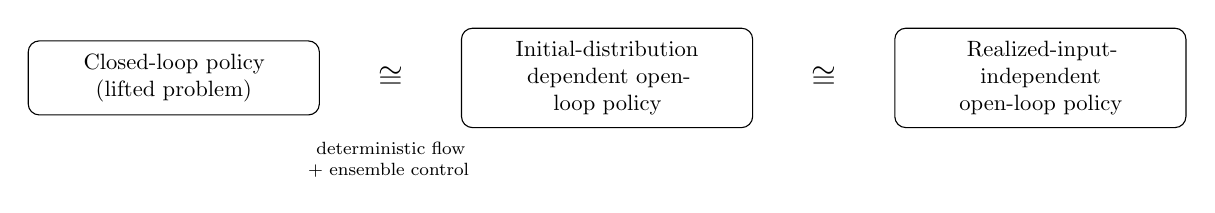
\begin{tikzpicture}[
          scale=0.8,
          transform shape,
          node distance=18mm,
          box/.style={draw, rounded corners, align=center, inner sep=6pt, text width=4.2cm},
          eq/.style={font=\Large},
          note/.style={font=\footnotesize, align=center, text width=4.8cm},
        ]
            \node[box] (cl) {Closed-loop policy\\(lifted problem)};
            \node[eq, right=8mm of cl] (e1) {$\cong$};
            
            \node[box, right=8mm of e1] (ol0) {Initial-distribution\\dependent open-loop policy};
            \node[note, below=6mm of e1] (why) {deterministic flow\\+ ensemble control};
            
            \node[eq, right=8mm of ol0] (e2) {$\cong$};
            
            \node[box, right=8mm of e2] (ol) {Realized-input-independent\\open-loop policy};
        \end{tikzpicture}
 \caption{Equivalence Properties of Control Policies for Transformer Design.}
\label{EquivalenceControlPol}
\end{figure}


    \item[(ii)] \textbf{Computational design via triply quantized learning scheme.} We propose a training procedure based on quantizing the particle state space, the measure space, and the action space. We show that this formulation gives rise to a finite state, finite action, measure-valued MDP, for which the computation of optimal policies via dynamic programming recursions is tractable. While establishing the existence of optimal policies for the triply quantized measure-valued MDP, we also provide a method for computing such policies (Theorem \ref{thm:triply-quantized-optimal-policies}) via dynamic programming recursions and then, we prove that any optimal policy for the triply quantized case is near-optimal for the original problem (Theorem \ref{thm:triply-quantized-efficiency}); please see Figure \ref{fig:model-hierarchy}. 
    \item[(iii)] \textbf{Robustness to training data, empirical consistency and asymptotic $\Gamma$-convergence to optimality.} By using a double-lifted formulation, which is a generalization of the lifted-formulation used for training, we establish the continuity of the cost functional with respect to the training data (Theorem \ref{thm:robustness}). This result provides an asymptotic answer to the generalization problem for Transformers.
\end{itemize} 
\begin{figure}[H]
\centering
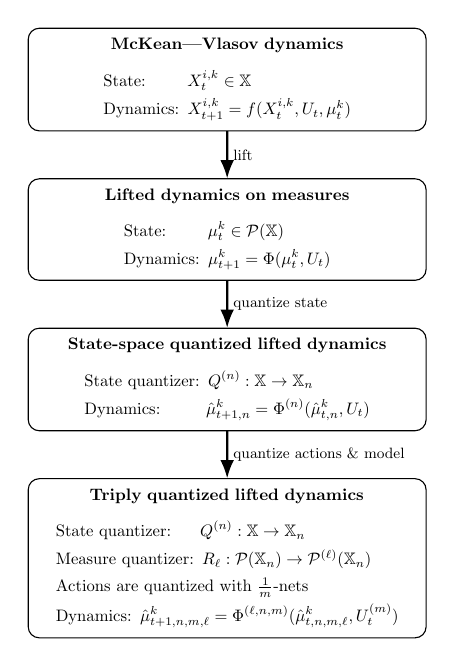
\begin{tikzpicture}[
    scale=0.6,
    transform shape,
    box/.style={draw, rounded corners, align=center, inner sep=6pt, text width=8cm},
    arr/.style={-Latex, thick},
    node distance=10mm,
]

\node[box] (base) {
\textbf{McKean---Vlasov dynamics}
\begin{align*}
    &\text{State: } \hspace{2em}X_t^{i,k}\in\XX\\
    &\text{Dynamics: } X_{t+1}^{i,k}=f(X_t^{i,k},U_t,\mu_t^k)
\end{align*}
};

\node[box, below=of base] (lift) {
\textbf{Lifted dynamics on measures}
\begin{align*}
    &\text{State: }  \hspace{2em}\mu_t^k \in \mathcal{P}(\XX)\\
    &\text{Dynamics: }\mu_{t+1}^k=\Phi(\mu_t^k,U_t)
\end{align*}
};

\node[box, below=of lift] (sq) {
\textbf{State-space quantized lifted dynamics}
\begin{align*}
    &\text{State quantizer: }Q^{(n)}:\XX\to\XX_n\\
    &\text{Dynamics: } \hspace{2.25em}\hat{\mu}_{t+1,n}^k=\Phi^{(n)}(\hat{\mu}_{t,n}^k,U_t)
\end{align*}
};

\node[box, below=of sq] (tq) {
\textbf{Triply quantized lifted dynamics}
\begin{align*}
    &\text{State quantizer: } \hspace{1.25em}Q^{(n)}:\XX\to\XX_n\\
    &\text{Measure quantizer: }R_\ell:\cP(\XX_n)\to\cP^{(\ell)}(\XX_n)\\
    &\text{Actions are quantized with $\textstyle\frac{1}{m}$-nets}\\
    &\text{Dynamics: }\hat{\mu}_{t+1,n,m,\ell}^k=\Phi^{(\ell,n,m)}(\hat{\mu}_{t,n,m,\ell}^k,U_t^{(m)})
\end{align*}
};

\draw[arr] (base) -- (lift) node[midway, right] {\small lift};
\draw[arr] (lift) -- (sq)   node[midway, right] {\small quantize state};
\draw[arr] (sq)   -- (tq)   node[midway, right] {\small quantize actions \& model};

\end{tikzpicture}
\caption{Four-level hierarchy of dynamics.}
\label{fig:model-hierarchy}
\end{figure}

\section{The Proposed Optimal Control Formulation of Transformers}\label{sec:formulation}
In this section, we interpret the forward dynamics of  Transformers as a discrete-time controlled dynamical system of interacting particles and show how the training procedure can be formulated as a finite-horizon optimal control problem. Since each particle evolves through the interactions with the empirical measure of the ensemble, the resulting dynamics is not Markovian at the particle level. The Markovian property is essential in our formulation of Transformers as an optimal control problem as it allows us to decompose the training problem into tractable and smaller subproblems using the dynamic programming principle, which guarantees the existence of optimal weights, and also provides a structural description of them.

In the work of \cite{geshkovski2025mathematical}, Transformers are described via the flow map of a continuous-time dynamical system. We adopt this approach, but, rather than considering the continuous-time system, we study a discrete-time version of the resulting dynamics that models a Transformer block with a feed-forward layer and single-headed self-attention. The formulation presented in this paper can be generalized to the multi-headed self-attention case. We therefore restrict ourselves to the single-headed self-attention for brevity and simplicity of the presentation. 

More precisely, we view Transformers as sequence-to-sequence maps and, motivated by the universal approximation result of \cite{yun2019transformers}, our goal is to identify an optimal Transformer architecture that best explains the training data. We assume that the data are generated, possibly in a noisy manner, by an underlying sequence-to-sequence mapping. For a meaningful comparison between input and output sequences, the position of each element must be preserved. To this end, we equip particles with positional encodings, which allow us to recover positional information after lifting the system to the space of probability measures in order to obtain a Markovian representation. Although this lifting breaks the exchangeability property, a mean-field analysis remains possible by exploiting the underlying McKean---Vlasov structure of the particle dynamics.
\medskip

\noindent\textbf{Notation.} We list the notation used throughout this paper.
\begin{itemize}
    \item $\mathrm{S}\subset\RR^d$, for some $d\in\NN$, denotes the state space of individual particles.
    \item Let $N\in\NN$ be the number of particles on which a Transformer acts. We denote the index set of particles by $\cN := \{1,\ldots,N\}$.
    \item $\beta > 0$ is a system-specific constant appearing in the self-attention block measuring the sensitivity of the dynamics to attention values between different particles.
    \item $T\in\NN$ is the time horizon. In the neural networks literature, $T$ corresponds to the number of layers. We denote the set of all layers by $\overline{\cT} := \{0,1,\ldots,T\}$ and the set of all layers except the output layer, or terminal state, by $\cT := \{0,1,\ldots,T-1\}$. The latter can also be called \emph{decision horizon}.
    \item $\mathrm{PE}_N := \{\frac{i}{N} : i\in\cN\}$ is the set of positional encodings.
    \item For a locally compact Polish space $\Omega$, $\cC_0(\Omega)$ denotes the set of all continuous functions from $\Omega$ to $\RR$ vanishing at infinity. We endow $\cC_0(\Omega)$ with the supremum norm that turns it into an $\RR$-Banach space. Moreover, $\cC_b(\Omega)$ is the set of all continuous and bounded functions from $\Omega$ to $\RR$. With the sup norm, $\cC_b(\Omega)$ is also an $\RR$-Banach space that has $\cC_0(\Omega)$ as a closed subspace.
    \item On the same Polish space $\Omega$ equipped with Borel $\sigma$-field $\cB(\Omega)$, $\cM(\Omega)$ denotes the space of all finite signed Borel measures on $(\Omega, \cB(\Omega))$. Furthermore, $\cP(\Omega)$ denotes the set of all probability measures on $(\Omega, \cB(\Omega))$.
    \item $S_N$ is the set of all bijections from $\cN$ to $\cN$.
\end{itemize}

\subsection{Transformer dynamics as a controlled particle system}
We present below the particle level dynamics of a Transformer block. For each $i\in\cN$, we have
\begin{equation}\label{eq:dynamics}
    \begin{cases}
        \displaystyle x_{t+1}^i = W_t\sigma(A_tx_t^i + b_t) + \sum_{j=1}^N \frac{ \e^{\beta\inner{Q_tx_t^i}{K_tx_t^j}}}{\sum_{j^\prime=1}^N\e^{\beta\inner{Q_tx_t^i}{K_tx_t^{j^\prime}}}}V_tx_t^j & \text{where } t\in\cT \\
        \displaystyle x^i_0 = x^i \in \mathrm{S}.
    \end{cases}
\end{equation}
The function $\sigma:\RR^{d_1}\to\RR^{d_1}$, $d_1\in\NN$, is called an \emph{activation function}. Usually, $\sigma$ is taken as a nonlinear function of $1$-Lipschitz class adding complexity and better approximation capabilities to the model. One of the most widely used activation functions is \emph{rectified linear unit} (ReLU) defined by $\operatorname{ReLU}(x^1,\ldots,x^{d_1}) = (\max\{x^1, 0\},\ldots,\max\{x^{d_1}, 0\})$ for all $(x^1,\ldots,x^{d_1})\in\RR^{d_1}$. In this formulation, the weights $W_t,A_t,b_t,Q_t,K_t,V_t$ are common to the entire ensemble at each time $t\in\cT$, and they are specified as $W_t\in\RR^{d\times d_1}$, $A_t\in\RR^{d_1\times d}$, $b_t\in\RR^d_1$, $Q_t, K_t\in\RR^{d_2\times d}$, and $V_t\in\RR^{d\times d}$ for some $d_1,d_2\in\NN$. For brevity, we occasionally write $U_t = (W_t,A_t,b_t,Q_t,K_t,V_t)$.
\begin{figure}[H]
    \centering
    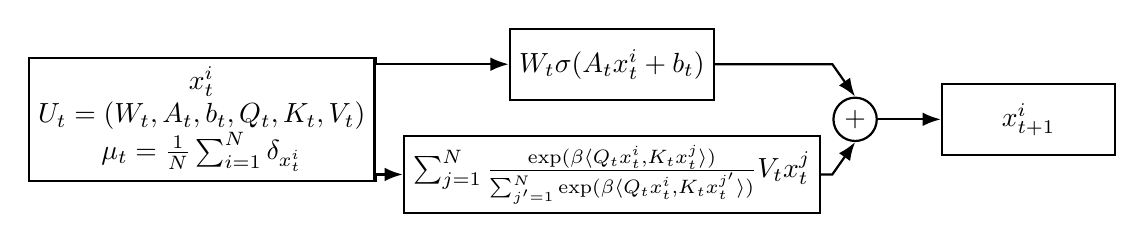
\begin{tikzpicture}[
  >=Latex,
  arr/.style={->, thick},
  block/.style={draw, rectangle, thick, align=center, minimum height=9mm, minimum width=22mm},
  bigblock/.style={draw, rectangle, thick, align=left, inner sep=6pt, minimum width=70mm},
  sum/.style={draw, circle, thick, inner sep=0pt, minimum size=5.5mm},
  lab/.style={align=left}
]

\node[block] (ff) {$W_t\sigma(A_tx_t^{i} + b_t)$};
\node[block, yshift=-14mm] (att) {$\sum_{j=1}^N \frac{ \operatorname{exp}(\beta\langle Q_tx_t^i,K_tx_t^j\rangle)}{\sum_{j^\prime=1}^N\operatorname{exp}({\beta\langle Q_tx_t^i,K_tx_t^{j^\prime}\rangle})}V_tx_t^j$};
\node[block, left=30mm of $(ff)!0.5!(att)$] (ing)  {$x_t^{i}$\\
$U_t=(W_t,A_t,b_t,Q_t,K_t,V_t)$ \\
$\mu_t=\frac{1}{N}\sum_{i=1}^N\delta_{x_t^{i}}$};

\node[sum, right=28mm of $(ff)!0.5!(att)$] (plus) {$+$};
\node[block, right=8mm of plus] (out) {$x_{t+1}^{i}$};

\draw[arr] (ing.north east) |- (ff.west);
\draw[arr] (ing.south east) |- (att.west);

\draw[arr] (ff.east) -- (plus.west |- ff.east) -- (plus.north);
\draw[arr] (att.east) -- (plus.west |- att.east) -- (plus.south);

\draw[arr] (plus.east) -- (out.west);

\end{tikzpicture}
\caption{Decompositional illustration of the flow \eqref{eq:dynamics}.}
\label{fig:eq1-compact-flow}
\end{figure}

As mentioned earlier, we regard a Transformer as an approximation of a sequence-to-sequence function $T:\mathrm{S}^N\to\mathrm{S}^N$. Unless this function is permutation invariant, which is typically not the case, the position of each particle plays an important role. Therefore, we pair each particle $x_t^i$ with a positional encoding $i/N\in\mathrm{PE}_N$ and form superstates $X_t^i = (i/N, x_t^i)$ for each $i\in\cN$ and all $t\in\overline{\cT}$. We henceforth write $p_i = i/N$ for each $i\in\cN$. Note that the positional encodings are time-independent, i.e. they are fixed throughout the time horizon. To this extent, we define the augmented dynamics as follows.
\begin{equation}\label{eq:augdynamics}
    \begin{cases}
        \displaystyle X_{t+1}^i := (p_i,x_{t+1}^i) = \left(p_i,W_t\sigma(A_tx_t^i + b_t) + \sum_{j=1}^N \frac{ \e^{\beta\inner{Q_tx_t^i}{K_tx_t^j}}}{\sum_{j^\prime=1}^N\e^{\beta\inner{Q_tx_t^i}{K_tx_t^{j^\prime}}}}V_tx_t^j\right) & \text{where } t\in\cT \\
        \displaystyle X_0^i = (p_i,x^i_0) = (p_i,x^i) \in \mathrm{PE}_N\times\mathrm{S}\\ 
    \end{cases}
\end{equation}
For brevity, we denote the state space of particles by $\XX$, that is $\XX := \mathrm{PE}_N\times\mathrm{S}$. We note that $\mathrm{PE}_N$ can be substituted with another finite set; for instance,  in the formulation of \cite{vaswani2017attention}, sinusoidal positional encodings are utilized. In comparison with a standard neural network, \(N\) typically represents the network \emph{width}; that is, the maximum number of nodes across all layers, and the width may vary from layer to layer. In contrast, our formulation assumes a fixed width throughout.

Considering the design of control actions, i.e. weights, one may choose \(d_1 > d\); in this case, the vectors \(Q_t x_t^i\) and \(K_t x_t^j\) take values in \(\mathbb{R}^{d_1}\). Accordingly, the matrices \(Q_t\) and \(K_t\) can be interpreted as linear projections onto the so-called \emph{query} and \emph{key} spaces, respectively. 

The dynamics \eqref{eq:augdynamics} define a discrete-time controlled dynamical system of interacting particles with shared actions. In the next part, we introduce the data set and the corresponding information structure of the optimal control problem.
\subsection{Data set-induced dynamics and information structure} In the classical training of Transformers, given some data set, the goal is to minimize some cost functional over the set of weights. We now formulate the corresponding scenario as an optimal control problem. To this end, suppose that we are given a data set $\cD := \{(\mathbf{x}^k, \mathbf{y}^k): k=1,2,\ldots,K\}\subseteq\mathrm{S}^N\times\mathrm{S}^N$, for some $K\in\NN$. In some applications, the learning goal is to approximate a classifier function $T:\mathrm{S}^N\to\cY$ where $\cY$ is a finite set of certain classifications. In such problems, the output vector is mapped to a class label by a known function. In our formulation, we consider the case in which Transformer maps feature vectors to label vectors, and the corresponding classes of the latter are known. Conceptually, this is equivalent to previously mentioned sequence-to-sequence function approximation paradigm and captures most learning scenarios.

For each $k\in\cK := \{1,\ldots,K\}$, the feature vector $\mathbf{x}^k = (x^{1,k},\ldots,x^{N,k})\in\mathrm{S}^N$ gives rise to an ensemble of particles $(X_t^{1,k},\ldots,X_t^{N,k})$ that evolves with \eqref{eq:augdynamics} with initial states $X_0^{i,k} = (p_i, x^{i,k})$ for each $i\in\cN$. In our problem, we consider a \emph{centralized information structure}
\begin{equation}
    \cI_t^{i,k} = \cI_t := \{X_s^{i, k}, U_s : i\in\cN, k\in\cK, 0 \leq s \leq t-1\}\cup\{X_t^{i, k} : i\in\cN, k\in\cK\}
\end{equation}
for all $t\in\overline{\cT}\setminus\{0\}$ and all $i\in\cN$. If $t=0$, we have $\cI_0 = \{X_0^{i,k}: i\in\cN, k\in\cK\}$. The equality $\cI_t^{i,k} = \cI_t$ indicates that each particle $X_t^{i,k}$ has access to the same information structure. In optimal control problems, the actions are chosen using a \emph{policy}, which is a sequence of either functions mapping the information structure to actions over the time horizon or stochastic kernels on actions given the information structure. However, choosing an action probabilistically is not compatible with Transformers since they work with concrete fixed weights. Therefore, we need policies of the form $(\gamma_t)_{t\in\cT}$ consisting of functions of the form $\gamma_t(\cI_t) = U_t\in\UU$ for each $t\in\cT$. In Section 3, we show that the choice of actions can be done in a deterministic way if we lift our problem to the space of probability measures. However, we subsequently show that the deterministic policies based on feedback (closed-loop policies) are not compatible with Transformers either. Therefore, we introduce the initial-condition-dependent open-loop policies obtained from closed-loop policies that are optimal and fully compatible with the usual training paradigm of Transformers.

We note that the choice of actions is not performed by a single particle or a group of particles that exclude some other particles. On the contrary, the choice is done by observing all of the ensembles. This is called an \emph{ensemble control problem} since we are trying to find optimal controls that are optimal for each member of the ensemble. 

The choice of information structure is intentional since we seek conformity with the current training configurations in which similar mechanisms are used. In the classical training of Transformers, the weights are trained using the information accumulated across all tokens and all samples, the controls in our formulation have to depend on all past information as well as the current information, which naturally results in a centralized information structure. This property of the centralized information structure is called the \emph{perfect recall} property, that is, we make decisions while having all possible information available. In general, an information structure might be more complicated, see the book of \cite{yuksel2024stochastic} for a detailed analysis of information structure-dependent properties of team optimal control problems.

In the next subsection, we complete our optimal control problem formulation of the training procedure of Transformers by introducing the cost functional and giving a sensible optimality criterion.

\subsection{Cost functional and optimality criterion}
Having specified the dynamics and the information structure, we now complete our formulation of Transformer training as an optimal control problem by defining a cost functional and the associated optimality criterion. In standard training, the objective is to minimize the empirical risk over the data set; in our formulation, we minimize a cost measuring the average discrepancy between the terminal states and the target vectors.

Let $\Gamma$ be the set of all admissible policies. For any $\underline{\gamma}\in\Gamma$, we write $x_{t,\underline{\gamma}}^{i,k}$ for the particle evolving according to \eqref{eq:dynamics} where the controls are obtained by $\underline{\gamma}$ and the centralized information structure we defined earlier. For the label vectors, we write $\mathbf{y}^k = (y^{1,k},\ldots,y^{N,k})$ for all $k\in\cK$. We compare the feature and label vectors using a loss function $L:\mathrm{S}\times\mathrm{S}\to\RR_+$. The minimization task is as follows
\begin{align*}
    &\underset{\displaystyle\underline{\gamma}\in\Gamma}{\text{minimize}}\quad\frac{1}{NK}\sum_{i=1}^N\sum_{k=1}^K L(x_{T,\underline{\gamma}}^{i,k}, y^{i,k}) \\
    &\text{subject to: } x_{t,\underline{\gamma}}^{i,k} \text{ evolving according to \eqref{eq:dynamics}},\\
    &\hspace{5em} x_{0,\underline{\gamma}}^{i,k} = x^{i,k} \text{ for all } i\in\cN, k\in\cK, t\in\cT. \tag{OP}\label{prob:original}
\end{align*}

In Section \ref{sec:robustness}, we discuss the robustness properties of the value function associated to the lifted formulation presented in Section \ref{sec:lifting-section}. This is the optimal control--theoretic analogue of the generalization problem in neural network. To this end, we provide another representation of the problem expressed as a finite-horizon terminal-cost-only expected cost functional minimization. Let $P_\cD$ denote the true distribution of the data set $\cD$, that is $P_\cD \in \cP(\mathrm{S}^N\times\mathrm{S}^N)$. For convenience, we write
\begin{equation*}
    \mathbf{L}(\mathbf{x}, \mathbf{y}) := \frac{1}{N}\sum_{i=1}^N L(x^i, y^i)
\end{equation*}
for all $\mathbf{x} := (x^1,\ldots,x^N)$, $\mathbf{y} := (y^1,\ldots,y^N) \in \mathrm{S}^N$. We consider a scenario in which the central controller try to find an policy that is optimal for the underlying distribution. 
\begin{align*}
    &\hspace{-3em}\underset{\displaystyle\underline{\gamma}\in\Gamma}{\text{minimize}}\quad\EE_{P_\cD}^{\underline{\gamma}}\mathbf{L}(\mathbf{x}_{T}, \mathbf{y}). \tag{ROP}\label{prob:robustness-original}
\end{align*}
Here $\mathbf{x}_T$ denotes the terminal state of the process, whose initial distribution is the first marginal of $P_\cD$, evolving in the trajectory specified by the Transformer dynamics \eqref{eq:dynamics} and by the policy $\underline{\gamma}\in\Gamma$.

There are several benefits of the presentation of the optimization problem as if the initial data is random: 
\begin{itemize}
\item[(i)] This captures the standard setup given in (OP) above, where the data is empirically given, in which case, the distribution is the realized empirical distribution for training. 
\item[(ii)] As noted, this allows us to formulate the robustness to initial training data and asymptotic consistency as the data converges weakly or in the Wasserstein sense to a true distribution based on which data is generated. 
\item[(iii)] This formulation makes the subtle point of open-loop/closed-loop policy discussion transparent: The policy we obtain is closed loop in the distribution, but open loop in the realization during the implementation of the Transformer for any source once the Transformer is trained.
\end{itemize}

In the definition of cost functional, we only consider feature vectors and omit positional encodings. Since $(p_i,x_{T,\underline{\gamma}}^{i,k})$ and $(p_i, y^{i,k})$ have the same positional encodings for all $i\in\cN$ and all $k\in\cK$, any sensible metric on $\mathrm{PE}_N$ would provide a zero contribution to the cost structure. The reason why we introduce the positional encodings is motivated by preserving the positional information while lifting the problem to probability measures.

In this paper, we primarily will consider the quadratic distance criterion, i.e.
\begin{equation}
    L(x,y) := \|x-y\|_2^2
\end{equation}
for all $x,y\in\mathrm{S}$, where $\|\cdot\|_2$ denotes the Euclidean norm on $\RR^d$. In practice, for example when training LLMs, the cost function differs from the one we use in this paper, see the contribution of \cite{phuong2022formal}. Such variations do not disturb the analysis presented this paper as long as we have a jointly continuous loss function. However, it may result in a different cost structure which might be computed along the time-horizon instead of a terminal-cost.

Although the cost function $(\mathrm{S}^N)^K\ni(x^{i,k})_{i\in\cN,k\in\cK}\mapsto\frac{1}{NK}\sum_{i=1}^N\sum_{k=1}^K\|x^{i,k}-y^{i,k}\|^2$ is strictly convex, the constraints given by Transformer dynamics \eqref{eq:dynamics} are highly nonconvex. Therefore, applying methods requiring convexity such as gradient descent can only guarantee convergence to local minima, and in general, do not provide guarantees of global optimality. In Section 4, we propose a quantization based training method guaranteeing near-optimality, which is not dependent on convexity, but rather requiring mild assumptions on the state and action spaces. 

\begin{definition}\label{def:optimality}
    A strategy $\underline{\gamma}^*\in\Gamma$ is called \emph{globally optimal} if it attains the minimum in (\ref{prob:original}).
\end{definition}

We conclude our formulation of Transformers as an optimal control problem by noting that the particle-level dynamics are not Markovian. Indeed, the evolution of each particle depends on the empirical measure of the ensemble through the self-attention mechanism in \eqref{eq:dynamics}. Therefore, the dynamic programming principle is not directly applicable with the current formulation. In the next section, we show that the particles have a McKean---Vlasov-type dynamics that can be lifted to the space of probability measures, which restores the Markovian property.

\section{McKean---Vlasov Structure and Measure-Valued MDP}\label{sec:lifting-section}
In Section \ref{sec:formulation}, we formulated an optimal control problem modeling Transformer training and argued that, after constructing superstates, the dynamics can be lifted to the space of probability measures, giving rise to a Markov decision process. In this section, we make this lifting explicit, and we establish that the topological requirements for the application of dynamic programming hold under some compactness assumptions.

In particular, we (i) formalize the deterministic McKean---Vlasov representation of the dynamics, (ii) lift the particle-level dynamics to the space of probability measures, (iii) verify the weak Feller property of the resulting transition kernel, (iv) prove the existence of optimal closed-loop policies, and (v) relate these closed-loop policies to initial-data-dependent open-loop policies from the viewpoint of implementation and conformity with the standard training paradigm.

\subsection{Deterministic McKean---Vlasov representation of the particles.} We begin with defining the function $f:\XX\times\UU\times\cP(\XX)\to\XX$ for all $(p,x)\in\XX$, $U = (W, A, b,$ $ Q, K, V) \in\UU$, and $\mu\in\cP(\XX)$ by
\begin{equation}\label{eq:McKean---Vlasov}
    f((p, x), U, \mu) := \left(p,  W\sigma(Ax + b) + \dfrac{1}{\int_\mathrm{S} \mu_\mathrm{S}(\de z) \e^{\beta\inner{Qx}{Kz}}}\int_\mathrm{S} \mu_\mathrm{S}(\de \tilde{z}) \e^{\beta\inner{Qx}{K\tilde{z}}}V\tilde{z}\right),
\end{equation}
which models the flow of a single particle. To make this concrete, take $(p,x) = (p_i, x_t^{i,k}) = X_t^{i,k}$, $U_t\in\UU$ as in \eqref{eq:augdynamics}, and $\mu_t^k = \frac{1}{N}\sum_{i=1}^N\delta_{(p_i,x_t^{i,k})}$ for all $i\in\cN$, $k\in\cK$, and $t\in\cT$. Then 
\begin{align*}
    f(X_t^{i,k}, U_t, \mu_t^k) &= \left(p_i, W_t\sigma(A_tx_t^{i,k} + b_t) + \frac{1}{\int_\mathrm{S}\mu_t^k(\de z)\e^{\beta\langle Q_tx_t^{i,k}, K_tz\rangle}}\int_S\mu_t^k(\de z)\e^{\beta\langle Q_tx_t^{i,k}, K_tz\rangle}V_tz\right)\\
    &= \left(p_i,  W_t\sigma(A_tx_t^{i,k} + b_t) + \sum_{j=1}^N \frac{ \e^{\beta\inner{Q_tx_t^{i,k}}{K_tx_t^{j,k}}}}{\sum_{r=1}^N\e^{\beta\inner{Q_tx_t^{i,k}}{K_tx_t^{r,k}}}}V_tx_t^{j,k}\right) = X_{t+1}^{i,k}.
\end{align*}
Note that the flow of any particle does not solely depend on its previous realizations, but it depends explicitly on the empirical of the ensemble $\mu_t^k$. This shows that the particles do not have a Markovian transition regime. The positional encodings are fixed in the definition of $f$ since they are not dynamical variables over the time horizon, but merely structural labels whose purpose is to preserve the order of the particles.

\subsection{The lifted system and its continuity properties.} We continue with precisely explaining the lifting procedure. Then, we prove that the underlying dynamics are continuous under the following assumption:
\begin{assume}\label{assume:compactness}
    The particles' state space $\mathrm{S}$ and the action space $\UU$ are compact.
\end{assume}
As discussed earlier, we justify Assumption \ref{assume:compactness} by widespread usage of compactly supported data in most applications for the state space $\mathrm{S}$. For the compactness of $\UU$, it can be viewed as a regularization of actions such as substituting $\UU$ with a closed, norm-bounded subset of it. In addition, compactness of $\mathrm{S}$ implies the compactness of $\XX$ since $\mathrm{PE}_N$ is finite set, and therefore, is compact in discrete topology. This observation is crucial since we endow the space of probability measures with the weak\textsuperscript{*}-topology, that is a sequence of probability measures $(\mu_n)_{n\in\NN}$ \emph{$\text{weak}^*$-convergent} to $\mu\in\cP(\XX)$ if, for any continuous and bounded $h:\XX\to\RR$, we have 
\begin{equation*}
    \int_\XX\mu_n(\de x)h(x) \xrightarrow{n\to\infty} \int_\XX\mu(\de x)h(x).
\end{equation*} 
Under Assumption \ref{assume:compactness}, one of the nicest properties of $\text{weak}^*$-topology is that $\cP(\XX)$ is compact. Moreover, we have many other choices for a suitable metric. In particular, we consider a modified version of $p$-Wasserstein distance, $p\in[1,+\infty)$, defined by
\begin{equation}\label{eq:p-wasserstein}
    W_{p,\lambda}(P,Q) := \inf_{\pi\in\Pi(P,Q)}\left(\int_{\XX\times\XX}\pi(\de X, \de Y) \|X-Y\|_{p,\lambda}^p \right)^{\frac{1}{p}}
\end{equation} 
where $\|X-Y\|_{p,\lambda}^p = \|x-y\|_p^p + \lambda|p-q|^p$, $X=(p,x), Y = (q,y)\in\XX$, $\lambda > 0$, and 
\begin{equation*}
    \Pi(P,Q) := \{\pi\in\cP(\XX\times\XX) : \pi(\cdot\times\XX) = P(\cdot) \text{ and } \pi(\XX\times\cdot) = Q(\cdot)\}.
\end{equation*}
Here $\Pi(P,Q)$ is the set of couplings of $P$ and $Q$, i.e., all joint probability measures on $\XX\times\XX$ such that the respective marginals of each $\pi\in\Pi(P,Q)$ are $P$ and $Q$. This set is always non-empty since it contains $P\otimes Q$. Moreover, $\Pi(P,Q)$ is compact whenever $\XX$ is since it is a closed subset of $\cP(\XX\times\XX)$, a compact space. Since the functional $\Pi(P,Q)\ni \pi \mapsto \int_{\XX\times\XX} h\ \de\pi$ is continuous for all $h\in\cC(\XX\times\XX)$, by Weierstrass theorem and the fact that $h(X,Y) = \|X-Y\|_\lambda^p$ is continuous for all $p\in[1,+\infty)$, there exists a $\pi^*\in\Pi(P,Q)$ such that $\pi^*$ minimizes \eqref{eq:p-wasserstein}. Here the value of $\lambda$ is critical for enforcing the model to take the positional information into account. Since $\mathrm{S}$ is compact, then for any $x,y\in\mathrm{S}$ and $p,q\in\mathrm{PE}_N$, we have
\begin{equation*}
    \|(p,x) - (q,y)\|_{p,\lambda}^p = \|x-y\|_p^p + \lambda|p-q|^p \leq \operatorname{diam}(\mathrm{S}, \|\cdot\|_p)^p + \lambda < +\infty.
\end{equation*}
The choice of $\lambda$ affects the behavior of the minimization problem in \eqref{eq:p-wasserstein}. If $\lambda$ becomes larger, then the choice of optimal product measure $\pi^*$ will prioritize minimizing the cost contribution of positional encodings, which is what we want since it tolerates the lost positional information in the correct way. Later, we provide an explicit bound for $\lambda$ to ensure this. Considering $p$, we are more interested in the case $p=2$ since it corresponds to minimizing the square loss, which is one of the most popular cost option in deep learning problems.

In our formulation in Section \ref{sec:formulation}, we have $K$-many samples from which we construct the empirical measures $\mu_0^k = \frac{1}{N}\sum_{i=1}^N\delta_{(p_i,x^{i,k})}$ for each $k\in\cK$. Note that this measure representation not only encodes the particle state information, but also the positional information. We define the map $\Phi:\cP(\XX)\times\UU\to\cP(\XX)$ for all $\mu\in\cP(\XX)$ and $U\in\UU$ by calculating the following push-forward measure
\begin{equation}\label{eq:measure-evolution}
    \Phi(\mu, U) := \mu\circ T_{\mu, U}^{-1}
\end{equation} 
where $T_{\mu, U}:\XX\to\XX$ is given by $T_{\mu, U}(X) := f(X,U,\mu)$ for all $X\in\XX$. This can be viewed as the discrete-time analogue of the continuity equation in \citep{geshkovski2025mathematical}. Consequently, we have a concrete functional representation of the measure flow in this particular ensemble controlled McKean---Vlasov system. It follows that, by a change of variables argument, for any measurable $g:\XX\to\RR$, $k\in\cK$ and $t\in\cT$, we have
\begin{align*}
    \int_\XX \Phi(\mu_t^{k}, U_t)(\de p, \de x)g(p,x) &= \int_\XX \mu_t^k\circ T_{\mu_t^k, U_t}^{-1}(\de p, \de x) g(p, x) \\
    &= \int_\XX\frac{1}{N}\sum_{i=1}^N \delta_{(p_i,x_t^{i,k})}(T_{\mu_t^k, U_t}^{-1}(\de p, \de x)) g(p,x) \\
    &= \frac{1}{N}\sum_{i=1}^N g(T_{\mu_t^k, U_t}(p_i,x_t^{i,k})) \\
    &= \frac{1}{N}\sum_{i=1}^N g(f((p_i,x_t^{i,k}), U_t, \mu_t^k)) \\
    &= \frac{1}{N}\sum_{i=1}^N g(p_i,x_{t+1}^{i,k}) = \int_\XX\mu_{t+1}^k(\de p, \de x) g(p,x).
\end{align*}
Thus, $\Phi(\mu_t^k, U_t) = \mu_{t+1}^k$ for all $t\in\cT$ and $k\in\cK$. This indicates that each empirical measure evolves with a Markovian structure. Since our objective is to minimize a cost criterion over all training data, and consequently, all empirical measures, we consider a multi-variable generalization of $\Phi$ as $\bm{\Phi}:\cP(\XX)^K\times\UU\to\cP(\XX)^K$ is given, for all $(\mu^1,\ldots,\mu^K)\in\cP(\XX)^K$ and $U\in\UU$, by
\begin{equation}\label{eq:ensemble-dynamics}
    \bm{\Phi}(\mu^1,\ldots,\mu^K; U) = (\Phi(\mu^1, U), \ldots, \Phi(\mu^K, U)).
\end{equation}
This generalization allows us to control the minimization problem over the data set, a similar approach can be found in \citep{E2019}. On the other hand, we can now see the ensemble process $((\mu_t^1,\ldots,\mu_t^K))_{t\in\overline{\cT}}$, initialized from the data set $\cD$ and evolving with $\bm{\Phi}$, as a deterministic and measure-valued Markov decision process. This ensemble view allows us to use a cost criterion to which all points in the data set contribute. To continue, we now establish the continuity of $\Phi$. To do this, since we construct $\Phi$ using $f$, we first need the continuity of $f$ under Assumption \ref{assume:compactness}.
\begin{proposition}\label{prop:continuity-of-mv}
    Under Assumption \ref{assume:compactness}, the function $f$ in \eqref{eq:McKean---Vlasov} is jointly continuous on $\XX\times\UU\times\cP(\XX)$ where $\cP(\XX)$ is endowed with $\text{weak}^*$-topology. 
\end{proposition}
\begin{proof}
    It is straightforward to see that $\mathrm{S}\ni x \mapsto W\sigma(Ax+b)$ is continuous. Since continuous functions form a vector space, it suffices to analyze the remaining term. Since $\mathrm{S}$ and $\UU$ are compact, then for any $x\in\XX$ and $U = (W, A, b, Q, K, V)\in\UU$, the function $\mathrm{S}\ni z\mapsto\e^{\beta\inner{Qx}{K\tilde{z}}}$ is bounded. Also, it is continuous. Therefore, for any sequence $(P_n)_{n\in\NN}$ in $\cP(\mathrm{S})$ $\mathrm{w}^*$-converging to $P^*\in\cP(\mathrm{S})$ we have
    \begin{equation*}
        \int_\mathrm{S} P_n(\de\tilde{z})\e^{\beta\inner{Qx}{K\tilde{z}}} \xrightarrow{n\to\infty}\int_\mathrm{S} P^*(\de\tilde{z})\e^{\beta\inner{Qx}{K\tilde{z}}}.
    \end{equation*}
    This convergence is uniform on compact subsets of the action space, which suffices for the entire action space under Assumption \ref{assume:compactness}. Of course, this statement is meaningful if we remind that if a sequence of probability measures $(\mu_n)_{n\in\NN}$ in $\cP(\XX) $ is $w^*$-convergent to $\mu^*\in\cP(\XX)$, then the marginal of each $\mu_n$ on $\mathrm{S}$ converges to the marginal of $\mu^*$ on $\mathrm{S}$ in $\text{weak}^*$-topology since the projection map is continuous \cite[Theorem 2.7]{billingsley2013convergence}. On the other hand, since $\mathrm{S}\ni z\mapsto\e^{\beta\inner{Qx}{K\tilde{z}}}$ is bounded and we are working on finite measures, dominated convergence theorem \cite[Theorem 2.4.5]{cohn2013measure} is applicable. Therefore, for any $Q^{(n)}\to Q$ in $\RR^{d\times k}$, $K_n\to K$ in $\RR^{d\times k}$, $x_n\to x$ in $\mathrm{S}$, we have
    \begin{equation*}
        \int_\mathrm{S}P(\de\tilde{z})\e^{\beta\inner{Q^{(n)}x_n}{K_n\tilde{z}}} \xrightarrow{n\to\infty}\int_\mathrm{S} P(\de\tilde{z})\e^{\beta\inner{Qx}{K\tilde{z}}}. 
    \end{equation*} 
    Note that this convergence is not dependent on the choice of measure $P$. Since we have uniform convergence in each separate argument, we have joint continuity.

    Next, we examine the continuity of $(\mu, Q, K, V, x) \mapsto \int_\mathrm{S} \mu_{\mathrm{S}}(\de \tilde{z}) \e^{\beta\inner{Qx}{K\tilde{z}}}V\tilde{z}$. It is important to see that the integration here is in the sense of Bochner integration in finite dimensions. The strong measurability of $(Q, K, V, x)\mapsto\e^{\beta\inner{Qx}{K\tilde{z}}}V\tilde{z}$ is routine and the continuity of the same function is an application of dominated convergence theorem for Bochner integration \cite[Theorem E.6]{cohn2013measure}. Since the continuous functions form an algebra, $f$ is (uniformly) continuous in the control argument $U$.
    
    Finally, it is immediate that $f$ is uniformly continuous in $p$. Therefore, $f$ is jointly continuous.
\end{proof}

As a consequent of Proposition \ref{prop:continuity-of-mv}, we establish the continuity of $\Phi$ in the next result.
\begin{proposition}\label{prop:phi-continuity}
    Under Assumption \ref{assume:compactness}, $\Phi$ defined in \eqref{eq:measure-evolution} is jointly continuous on $\cP(\XX)\times\UU$.
\end{proposition}
\begin{proof}
    First, we show the uniform convergence in each separate argument. Let $(\mu_n)_{n\in\NN}$ be a sequence in $\cP(\XX)$ that is $W_{1,\lambda}$-convergent to $\mu\in\cP(\XX)$. The topology generated by $W_{1,\lambda}$ is equivalent with $W_{2,\lambda}$ for compact state space. For simplicity, write $X$ for the generic element of $\XX$. Then, for any $g:\XX\to\RR$ with minimal Lipschitz constant $1$ and $U\in\UU$, we have
    \begin{align*}
        \bigg|\int_\XX (\Phi(\mu_n, U)-\Phi(\mu, U))(\de p, \de x) g(p,x)\bigg| &=  \bigg|\int_\XX \mu_n(\de p, \de x) g(T_{\mu_n, U}(p,x)) \\
        &\hspace{5em}-\int_\XX \mu(\de p, \de x)g(T_{\mu, U}(p, x))\bigg|\\
        &\leq \bigg|\int_\XX\mu_n(\de p, \de x) \big(g(T_{\mu_n, U}(p,x)) \\
        &\hspace{10em}- g(T_{\mu,U}(p,x))\big)\bigg| \\
        &\quad+ \bigg|\int_\XX (\mu_n-\mu)(\de p,\de x)g(T_{\mu, U}(p,x))\bigg|\\
        &\leq \int_\XX \mu_n(\de p, \de x)|g(f(p,x; U, \mu_n))\\
        &\hspace{10em}-g(f(p,x; U, \mu))| \\
        &\quad+\int_\XX|\mu_n-\mu|(\de p, \de x)|g(f(p,x; U, \mu))|\\
        &\leq \sup_{(p,x)\in\XX}|f(p,x; U, \mu_n) - f(p,x; U, \mu)|\\
        &\qquad+ \|g\|_{\infty}W_{1,\lambda}(\mu_n, \mu)
    \end{align*}
    where the last inequality is due to the Lipschitz property of $g$ and the definition of $W_{1,\lambda}$ distance. Since $\mu_n\xrightarrow{W_{1,\lambda}}\mu$ and $f$ is continuous by Proposition \ref{prop:continuity-of-mv}, we have uniform convergence in $\cP(\XX)$.

    Now let $U_n\to U$ in $\UU$ and $\mu\in\cP(\XX)$ be arbitrary. Then,
    \begin{align*}
        \bigg|\int_\XX (\Phi(\mu, U_n)-\Phi(\mu, U))(\de p, \de x) g(p,x)\bigg| &= \bigg|\int_\XX \mu(\de p, \de x) g(T_{\mu, U_n}(p,x))\\
        &\hspace{7em}-\int_\XX \mu(\de p,\de x)g(T_{\mu, U}(p,x))\bigg| \\
        &\leq \int_\XX \mu(\de p, \de x) |g(T_{\mu, U_n}(p,x)) - g(T_{\mu, U}(p,x))| \\
        & \leq \sup_{(p,x)\in\XX}|f(p,x; U_n, \mu) - f(p,x; U, \mu)|.
    \end{align*}
    By the continuity of $f$ again, we have the uniform convergence in $\UU$ as well.
    Therefore, $\Phi$ is indeed jointly continuous on $\cP(\XX)\times\UU$ since it is uniformly continuous in each argument.  
\end{proof}

\noindent For $(\mu_t^1,\ldots,\mu_t^K)_{t\in\overline{\cT}}$, we define its transition kernel $\eta$ by
\begin{align}\label{eq:transition-kernel}
    \eta(B \mid \mu_t^1,\ldots,\mu_t^K; U_t) &:= \PP((\mu_{t+1}^1,\ldots,\mu_{t+1}^K)\in B \mid \mu_t^1,\ldots,\mu_t^K; U_t)\\
    &= \PP\{\bm{\Phi}(\mu_t^1,\ldots,\mu_t^K; U_t) \in B\} = \delta_{\bm{\Phi}(\mu_t^1,\ldots,\mu_t^K; U_t)}(B),
\end{align}
where $B\in\cB(\cP(\XX)^K)$. Here, we endow $\cP(\XX)^K$ with the product $\text{weak}^*$-topology and obtain the Borel $\sigma$-field structure.

Note that the continuity of $\Phi$ implies the continuity of $\bm{\Phi}$, which is critical since we want the transition kernel $\eta$ to be \emph{weak Feller}, that is, for any continuous and bounded function $g:\cP(\XX)^K\to\RR$, we have
\begin{equation}\label{eq:weak-feller}
    \cP(\XX)^K\times\UU\ni(\mu^1,\ldots,\mu^K; U)\mapsto\int_{\cP(\XX)^K}\eta(\de\mu_{t+1}^1,\ldots,\de\mu_{t+1}^K \mid \mu^1,\ldots,\mu^K; U)g(\mu_{t+1}^1,\ldots,\mu_{t+1}^K)
\end{equation}
is a continuous function. The next assertion, which is a corollary to \ref{prop:phi-continuity}, indeed verifies this hypothesis.
\begin{corollary}\label{cor:transition-kernel}
    The transition kernel $\eta$ defined in \eqref{eq:transition-kernel} is weak Feller under Assumption \ref{assume:compactness}.
\end{corollary}
\begin{proof}
    Due to Proposition \ref{prop:phi-continuity}, $\Phi$ is jointly continuous. Therefore, so is $\bm{\Phi}$. Then, let $(\bm{\mu}_n)_{n\in\NN}$ be a sequence in $\cP(\XX)^K$ converging to $\bm{\mu}\in\cP(\XX)^K$ in weak$^*$-topology and $(U_n)_{n\in\NN}$ be another sequence in $\UU$ converging to $U\in\UU$. Then for any continuous and bounded $g:\cP(\XX)^K\to\RR$, we have
    \begin{align*}
        \int_{\cP(\XX)^K} \eta(\de\bm{\mu}_{t+1}\mid \bm{\mu}_n; U_n)g(\bm{\mu}_{t+1}) &= \int_{\cP(\XX)^K}\delta_{\bm{\Phi}(\bm{\mu}_n, U_n)}(\de\bm{\mu}_{t+1})g(\bm{\mu}_{t+1}) \\
        &= g(\bm{\Phi}(\bm{\mu}_n, U_n))
    \end{align*}
    for all $n\in\NN$. Since both $g$ and $\Phi$ are continuous, we have
    \begin{equation*}
        \lim_{n\to\infty}g(\bm{\Phi}(\bm{\mu}_n, U_n)) = g(\bm{\Phi}(\bm{\mu}, U)) = \int_{\cP(\XX)^K} \eta(\de\bm{\mu}_{t+1}\mid \bm{\mu}; U)g(\bm{\mu}_{t+1}).
    \end{equation*}
    Thus, $\eta$ is weak Feller.
\end{proof}

\subsection{Existence of optimal policies}\label{sub:existence-of-optimality}
We now employ the framework of Markov decision processes. First, we observe that the ensemble of empirical measures $\left((\mu_t^1,\ldots,\mu_t^K)\right)_{t\in\overline{\cT}}$ is a Markov decision process defined on $\cP(\XX)^K$ with the action space $\UU$ where
\begin{itemize}
    \item $\cP(\XX)^K$ is endowed with the product $\text{weak}^*$-topology.
    \item for any $\bm{\mu}\in\cP(\XX)^K$ and $U\in\UU$, the transition kernel is given by
    \begin{equation}
    \eta(\cdot|\bm{\mu}, U) = \delta_{\bm{\Phi}(\bm{\mu}, U)}(\cdot).
    \end{equation}
    \item Our aim is to minimize the  following cost functional:

\begin{equation}\label{eq:cost-functional}
    V(\cD; \underline{\gamma}) =\frac{1}{K}\sum_{k=1}^K W_{2,\lambda}(\mu_T^k, \nu^k)^2
\end{equation}
over the set of all strategies $\Gamma$ for Transformers, where $\mu_T^k$ is initialised from the $k^{\text{th}}$-sample of the data set $\cD$ according to the flow $\Phi$ using the policy $\underline{\gamma}$. Moreover, $\nu^k := \frac{1}{N}\sum_{i=1}^N\delta_{(p_i,y^{i,k})}$ and
\begin{equation}
    W_{2,\lambda}(P, Q) := \left(  \inf_{\pi\in\Pi(P,Q)}\int_{\XX\times\XX}\pi(\de X, \de Y)c_\lambda(X,Y)^2 \right)^{\frac{1}{2}}
\end{equation}
for all $P,Q\in\cP(\XX)$. Recall the definition $\Pi(P,Q) := \{\pi\in\cP(\XX\times\XX) : \pi(\cdot \times \XX) = P(\cdot), \pi(\XX\times\cdot) = Q(\cdot)\}$.
\end{itemize}
We define the cost function for $W_{2,\lambda}$-distance as
\begin{equation*}
    c_\lambda(X,Y) := \sqrt{\|x-y\|_2^2 + \lambda |p-q|^2}
\end{equation*}
where $X=(p,x), Y=(q,y)\in\XX$. To guarantee that we choose the correct $\pi^*\in\Pi(P,Q)$, i.e. the optimal one preserving positions, we first consider the following estimate for $p\neq q$:
\begin{align*}
    c_\lambda(X, Y) &= \|x-y\|_2^2 + \lambda |p-q|^2 \\
    &\leq \operatorname{diam}(\mathrm{S}, \|\cdot\|_2)^2 + \lambda|p-q||p+q|\\
    &\leq \operatorname{diam}(\mathrm{S}, \|\cdot\|_2)^2 + 2\frac{\lambda}{N}
\end{align*}
where $\operatorname{diam}(\mathrm{S}, \|\cdot\|_2) := \sup_{x,y\in\mathrm{S}}\|x-y\|_2$. If we choose $\lambda > \frac{N}{2}\operatorname{diam}(\mathrm{S}, \|\cdot\|_2)^2$, then enforce the rule that $\pi^*$ should minimize the positional encodings first in order to attain the infimum. We omit $\|\cdot\|_2$ from the notation that we previously used for $\operatorname{diam}$ since it is redundant as we are only interested in $2$-norm. In the next theorem, we establish the equivalence of the lifted problem and the original problem
\begin{theorem}
    If $\lambda > \frac{N}{2}\operatorname{diam}(\mathrm{S}, \|\cdot\|_2)^2$, then the lifted problem and (OP) are equivalent.
\end{theorem}
\begin{proof}
    Let $\bm{\mu}_{T,\underline{\gamma}} = (\mu_{T,\underline{\gamma}}^1,\ldots,\mu_{T,\underline{\gamma}}^K)$ be a generic terminal state evolved with $\bm{\Phi}$ under strategy $\underline{\gamma}\in\Gamma$ and initialized from the data set $\cD$. Respectively, let $\bm{\nu} := (\nu^1,\ldots,\nu^K)$ be the lifted labels, that is $\nu^k := \frac{1}{N}\sum_{i=1}^N\delta_{p_i, y^{i,k}}$ for all $k\in\cK$.

    In our case, where we compare empirical measures with the same number of atoms, the Wasserstein distance reduces to finding an optimal permutation. In particular, the optimal cost functional takes the form
    \begin{align*}
        V^*(\cD) &:= \inf_{\underline{\gamma}\in\Gamma}\frac{1}{K}\sum_{k=1}^K W_{2,\lambda}(\mu_{T,\underline{\gamma}}^k,\nu^k)\\
        &=\inf_{\underline{\gamma}\in\Gamma}\frac{1}{K}\sum_{k=1}^K \inf_{\sigma\in S_N}\frac{1}{N}\sum_{i=1}^N(\|x_{T,\underline{\gamma}}^{i,k} - y^{\sigma(i), k}\|_2^2 + \lambda|p_i - p_{\sigma(i)}|^2)
    \end{align*}
    Due to the choice of $\lambda$, we must have $\sigma$ as the identity permutation. Thus, we get
    \begin{equation*}
        V^*(\cD) = \inf_{\underline{\gamma}\in\Gamma}\frac{1}{NK}\sum_{k=1}^K \|x_{T,\underline{\gamma}}^{i,k} - y^{i, k}\|_2^2.
    \end{equation*}
    Recalling Definition \ref{def:optimality} concludes the proof.
\end{proof}

We impose the following assumption in order to have a position-sensitive cost structure.

\begin{assume}\label{assume:lambda}
    The choice of $\lambda$ is done in a way that $\lambda > \frac{N}{2}\operatorname{diam}(\mathrm{S}, \|\cdot\|_2)^2$ holds.
\end{assume}

Note that, we have written $V$ in a way it depends on the initial data. Since the problem is fixed for a given data set, we omit it and simply write $V(\underline{\gamma})$ for the same cost. In this expectation, we start with an ensemble of initial empirical measures, i.e. $\mu_0^k := \frac{1}{N}\sum_{i=1}^N\delta_{X_0^{i,k}}$ for all $k\in\cK$, and we transport the ensemble via $\bm{\Phi}$

\begin{figure}[H]
\centering
\resizebox{0.95\linewidth}{!}{
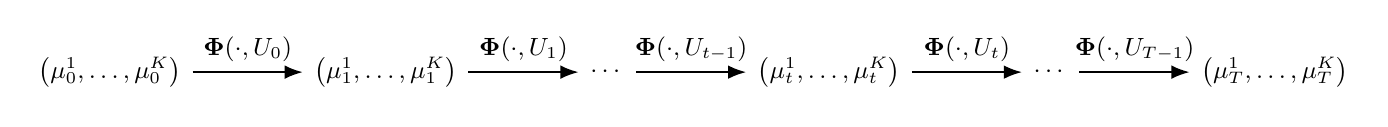
\begin{tikzpicture}[
  node distance=7mm,
  box/.style={rounded corners, align=center, inner sep=4pt, font=\small},
  arr/.style={-Latex, thick}
]
\node[box] (t0) {$\big(\mu_0^1,\ldots,\mu_0^K\big)$};

\node[box, right=14mm of t0] (t1) {$\big(\mu_{1}^1,\ldots,\mu_{1}^K\big)$};

\node[box, right=14mm of t1] (dots) {$\cdots$};

\node[box, right=14mm of dots] (t) {$\big(\mu_t^1,\ldots,\mu_t^K\big)$};

\node[box, right=14mm of t] (dots2) {$\cdots$};

\node[box, right=14mm of dots2] (T) {$\big(\mu_{T}^1,\ldots,\mu_{T}^K\big)$};

\draw[arr] (t0) -- node[above, font=\small] {$\boldsymbol{\Phi}(\cdot, U_0)$} (t1);
\draw[arr] (t1) -- node[above, font=\small] {$\boldsymbol{\Phi}(\cdot, U_1)$} (dots);
\draw[arr] (dots) -- node[above, font=\small] {$\boldsymbol{\Phi}(\cdot, U_{t-1})$} (t);
\draw[arr] (t) -- node[above, font=\small] {$\boldsymbol{\Phi}(\cdot, U_{t})$} (dots2);
\draw[arr] (dots2) -- node[above, font=\small] {$\boldsymbol{\Phi}(\cdot, U_{T-1})$} (T);
\end{tikzpicture}
}

\caption{Flow of the ensemble of empirical measures on particle via the map $\bm{\Phi}$.}
\label{fig:phi-bold-map}
\end{figure}
under $\underline{\gamma}\in\Gamma$. The choice of a variation of the $W_2$ distance is motivated by the fact that $\mathrm{PE}_N\times\RR^d$ can be endowed with the norm $\|\cdot\|_{2,\lambda}$ that generates the canonical topology on $\mathrm{PE}_N\times\RR^d$. Finally, we note the following properties of the cost structure. For any $\pi\in\cP(\XX\times\XX)$, we have
\begin{equation*}
    \int_{\XX\times\XX}c_\lambda^2\de\pi \leq \sup_{(X,Y)\in\XX\times\XX}c_\lambda(X,Y)^2\int_{\XX\times\XX}\de\pi = \sup_{(X,Y)\in\XX\times\XX}c_\lambda(X,Y)^2 \leq \operatorname{diam}(\mathrm{S})^2 + 2\frac{\lambda}{N} < +\infty.
\end{equation*}
Therefore, the cost structure is bounded. Since the metric $c_\lambda$ is jointly continuous (by the reverse triangle inequality), we also have the continuity of the cost function. 
\begin{remark}\label{remark:properties-of-transformers}
    Under Assumption \ref{assume:compactness}, we have
    \begin{itemize}
        \item[(R1)] The transition kernel $\eta$ is weak Feller by Corollary \ref{cor:transition-kernel}.
        \item[(R2)] The terminal cost function for Transformers, given by
        \begin{equation*}
            \cP(\XX)^K\ni(\mu^1,\ldots,\mu^K)\mapsto\frac{1}{K}\sum_{k=1}^K W_{2,\lambda}(\mu^k,\nu^k)^2
        \end{equation*}
        is continuous and bounded. 
    \end{itemize}
\end{remark}
There are several information structures that could be used in this problem. We previously mentioned the centralized information structure for the particle-level problem. For the lifted model, we have two main ISs to consider
\begin{enumerate}
    \item (\emph{Perfect recall}) $\cI_{t,\text{History}} := \{\mu_s^k, U_s : 0 \leq s \leq t-1, k\in\cK\}\cup \{\mu_t : k\in\cK\}$ for all $t\in\cT$.
    \item (\emph{State-feedback} or \emph{Markovian}) $\cI_{t,\text{Markovian}} := \{\mu_t^k : k\in\cK\}$ for all $t\in\cT$.
\end{enumerate}
Due to the Markovian flow of the ensemble and by Blackwell's theorem on the redundancy of information beyond the state \citep{blackwell1964memoryless}, it is enough to consider $\cI_{t,\text{Markovian}}$ and the deterministic Markovian policies among all admissible policies under centralized information structures. We denote the deterministic Markovian policies by $\Gamma$ from now on. 

\begin{theorem}\label{thm:transformers-optimality}
    Let Assumptions \ref{assume:compactness} and \ref{assume:lambda} hold. Let us define the dynamic programming equations
    \begin{equation}
        \begin{cases}
            \displaystyle\fC_T(\mu^1,\ldots,\mu^K) :=  \frac{1}{K}\sum_{k=1}^K W_{2,\lambda}(\mu^k,\nu^k)^2 \\
            \displaystyle\fC_t(\mu^1,\ldots,\mu^K) := \inf_{U\in\UU}\int_{\cP(\XX)^K}\eta(\de\mu_{t+1}^1,\ldots,\de\mu_{t+1}^K|\mu^1,\ldots,\mu^K; U)\fC_{t+1}(\mu_{t+1}^1,\ldots,\mu_{t+1}^K) \text{ for all $t\in\cT$},
        \end{cases}
    \end{equation}
    $\text{for all } (\mu^1,\ldots,\mu^K)\in\cP(\XX)^K$. Then there exists $\underline{\gamma}^*\in\Gamma$ such that
    \begin{equation}
        V(\underline{\gamma}^*) = \inf_{\underline{\gamma}\in\Gamma}V(\underline{\gamma})
    \end{equation}
    and $\underline{\gamma}^* = (\gamma_t^*)_{t\in\cT}$ is of class deterministic Markov in the sense that $\gamma_t^*(\mu_t^1,\ldots\mu_t^K) = U_t^*\in\UU$.
\end{theorem}
\begin{proof}
    This result directly follows from the analysis performed in \cite[Chapter 2]{hernandez2012discrete} in which the conditions for this case are satisfied via Assumption \ref{assume:compactness} and Remark \ref{remark:properties-of-transformers}.
\end{proof}
Note that, we could have written the dynamic programming equations in an equivalent way as follows: For any $t\in\cT$ and $\mu^1,\ldots,\mu^K\in\cP(\XX)$, we have
\begin{align*}
    \fC_t(\mu^1,\ldots,\mu^K) &= \inf_{U\in\UU}\int_{\cP(\XX)^K}\eta(\de\mu_{t+1}^1,\ldots,\de\mu_{t+1}^K|\mu^1,\l,dots\mu^K; U)\fC_{t+1}(\mu_{t+1}^1,\ldots\mu_{t+1}^K) \\
    &= \inf_{U\in\UU}\fC_{t+1}(\bm{\Phi}(\mu^1,\ldots,\mu^K; U))
\end{align*}
and in particular
\begin{align*}
    \fC_{T-1}(\mu^1,\ldots,\mu^K) &= \inf_{U\in\UU}\fC_T(\bm{\Phi}(\mu^1,\ldots,\mu^K; U))\\
    &= \inf_{U\in\UU}\sum_{k=1}^K W_{2,\lambda}(\Phi(\mu^k, U),\nu^k)^2.
\end{align*}
By induction, if we continue, we eventually have
\begin{equation*}
    V^* = \fC_0(\mu_0^1,\ldots,\mu_0^K) = \inf_{U_0\in\UU}\inf_{U_1\in\UU}\cdots\inf_{U_{T-1}\in\UU}\sum_{k=1}^KW_{2,\lambda}(\Phi(\Phi(\cdots\Phi(\mu_0^k, U_0),U_1),\cdots,U_{T-1})), \nu^k)^2.
\end{equation*}
With dynamic programming, we first minimize starting from inside to outside, meaning that we first minimize starting from the terminal cost. At each time-step, we work with only optimization of one term and get optimal control action for each state. If we select (measurably) one optimal control action for each state, we obtain so-called a deterministic Markovian policy; a function deterministically assigns a control according to only the information available at the same time-step. This procedure is more efficient than checking each action individually even if we have a finite set of admissible actions. However, we have a continuum of actions, which is not quite easy to work with currently. In the next section, we reduce this set to a finite one at the cost of having near-optimality. However, by doing this, we depend on the compactness of state and action spaces instead of relying on the convexity and smoothness of the problem, which is not the case in most applications.

\subsection{Open-loop policy design via closed-loop policy design for the lifted problem.}
Let $\underline{\gamma}^*\in\Gamma$ be a deterministic Markov strategy obtained from the dynamic programming equations. Although, with infinite state and action spaces, calculation of $\underline{\gamma}^*$ is very difficult, it corresponds to the training phase in classical approach. In the next section, we provide an approach to train Transformers with dynamic programming using quantization. 

We now discuss why open-loop policies constitute the appropriate class of policies in the context of Transformers. An \emph{open-loop} policy refers to a collection of control actions $(U_t)_{t\in\cT}$ for all $t\in\cT$. In other words, an open-loop policy is a finite sequence in the action space. A \emph{closed-loop} policy, also called \emph{feedback} policy, is given by a sequence of measurable maps $(\gamma_t)_{t\in\cT}$ of the form $\gamma_t(\mu_t^1,\ldots,\mu_t^K) = U_t\in\UU$ for all $t\in\cT$. Basically, a closed-loop policy yields an action based on the current state. 

In the operational context of Transformers, one would like to fix the architecture after the training process is finished. For example, if we were to use gradient descent for training provided that it is feasible to use it, we would have terminated the process when the gradient of loss function with respect to actions vanishes. Then, we would have a collection of actions, and whenever we feed some other data, the system returns an output by running the model with the weights obtained from that gradient descent-based training. This is exactly an open-loop policy since weights are not subject to change when the system is given a new data. However, in the case of closed-loop policies, the controls are calculated at each layer $t\in\cT$, which is not computationally efficient, and also, not compatible with classical paradigm.

We establish and build on the following equivalence for classes policies:
\begin{center}
 A {\it closed-loop policy of the lifted problem} is equivalent to an {\it initial-distribution dependent open-loop policy} (owing to the deterministic and ensemble nature of the lifted problem), which is, in turn, equivalent to a {\it realized-input-independent open loop policy}, and thus compatible with Transformer design (see Figure \ref{EquivalenceControlPol}). 
\end{center}

Again let $\underline{\gamma}^*\in\Gamma$ be an optimal closed-loop for the lifted model obtained via Theorem \ref{thm:transformers-optimality}. For $t=1$, we may write
\begin{equation*}
    U_1^* = \gamma_1^*(\mu_1^1,\ldots,\mu_1^K) = \gamma_1^*(\bm{\Phi}(\mu_0^1,\ldots,\mu_0^1; \gamma_0^*(\mu_0^1,\ldots, \mu_0^K))).
\end{equation*}
In other words, once we learn $\gamma_0^*$ and $\gamma_1^*$, we can calculate optimal action $U_1^*$ using only the initial data. By induction, it is possible to find functions $g_0^*,\ldots,g_T^*:\cP(\XX)^K\to\UU$ by, for any $t\in\cT$, we expand
\begin{align*} 
    U_t^* &= \gamma_t^*(\mu_t^1,\ldots,\mu_t^K) \\
    &=\gamma_t^*(\bm{\Phi}(\mu_{t-1}^1,\ldots,\mu_{t-1}^K;\gamma_{t-1}^*(\mu_{t-1}^1,\ldots,\mu_{t-1}^K)))\\
    &\hspace{1cm}\vdots\\
    &=\gamma_t^*(\bm{\Phi}(\cdots\bm{\Phi}(\mu_0^1,\ldots, \mu_0^K;\gamma_0^*(\mu_0^1,\ldots, \mu_0^K), \gamma_1^*(\bm{\Phi}(\mu_0^1,\ldots, \mu_0^K;\gamma_0^*(\mu_0^1,\ldots, \mu_0^K))\cdots))))\\
    &=: g_t^*(\mu_0^1,\ldots,\mu_0^K).
\end{align*}

\begin{figure}[H]
\centering
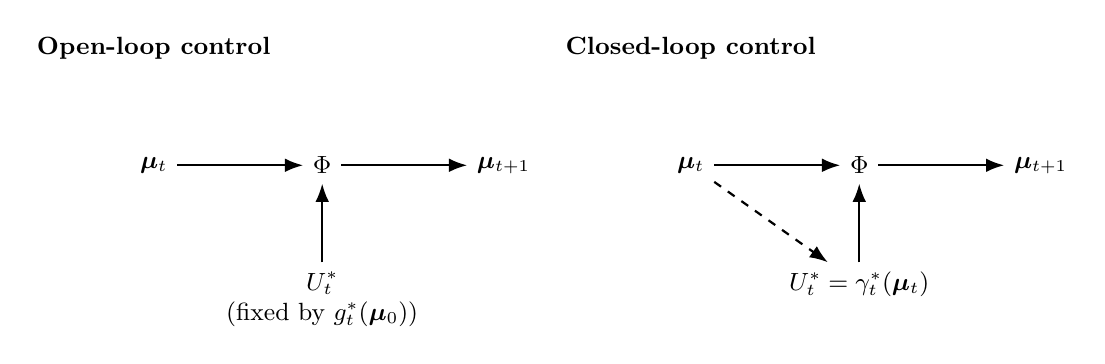
\begin{tikzpicture}[
    scale=1,
    transform shape,
  arr/.style={-Latex, thick},
  lab/.style={font=\small, align=center},
  node distance=10mm and 16mm
]

% ===== OPEN LOOP =====
\node[lab] (ol_title) {\textbf{Open-loop control}};
\node[lab, below=of ol_title] (ol_mu) {$\bm{\mu}_{t}$};
\node[lab, right=of ol_mu] (ol_phi) {$\Phi$};
\node[lab, below=of ol_phi] (ol_u) {$U_t^*$\\(fixed by $g_t^*(\bm{\mu}_{0})$)};
\node[lab, right=of ol_phi] (ol_mu_next) {$\bm{\mu}_{t+1}$};

\draw[arr] (ol_mu) -- (ol_phi);
\draw[arr] (ol_phi) -- (ol_mu_next);
\draw[arr] (ol_u) -- (ol_phi);

% ===== CLOSED LOOP =====
\node[lab, right=35mm of ol_title] (cl_title) {\textbf{Closed-loop control}};
\node[lab, below=of cl_title] (cl_mu) {$\bm{\mu}_{t}$};
\node[lab, right=of cl_mu] (cl_phi) {$\Phi$};
\node[lab, below=of cl_phi] (cl_u) {$U_t^*=\gamma_t^*(\bm{\mu}_{t})$};
\node[lab, right=of cl_phi] (cl_mu_next) {$\bm{\mu}_{t+1}$};

\draw[arr] (cl_mu) -- (cl_phi);
\draw[arr] (cl_phi) -- (cl_mu_next);
\draw[arr] (cl_u) -- (cl_phi);
\draw[arr, dashed] (cl_mu) -- (cl_u);

\end{tikzpicture}
\caption{Comparison of information structures for open-loop and closed-loop controls. In the open-loop case, $U_t^*$'s are fixed before and do not depend on the current measure unlike the closed-loop case.}
\label{fig:open-vs-closed}
\end{figure}

In short, by recursively expanding the expression $\gamma_t^*(\mu_t^1,\ldots,\mu_t^K)$ using the flow $\bm{\Phi}$ and preceding $\gamma_0^*,\ldots,\gamma_{t-1}^*$, we express $U_t^*$ as a function $F_t$ of $\mu_0^1,\ldots, \mu_0^K$ and $\gamma_0^*,\ldots,\gamma_{t-1}^*$. Then, we simply call it $g_t^*$. This collection of maps $(g_t^*)_{t\in\cT}$ is classified as an \emph{initial condition-dependent open-loop policy}. Since $\Phi$ and $\gamma_t^*$'s are deterministic, so is each $g_t^*$. Moreover, since $\Phi$ is known \emph{a priori} and $(\gamma_t^*)_{t\in\cT}$ is learned via dynamic programming, we know how to calculate each $g_t^*$. Therefore, we do not need to calculate actions at each time-step, which allows us to fix the architecture once we finish the training phase, as intended. Then, whenever new data is fed into the trained Transformer, the corresponding output will be given with the learned controls, or weights as it is done with the classical methods.

\section{Triply Quantized Training Scheme for Transformers}\label{sec:quantization}
We have so far developed a mathematical framework and control theoretic formulation on optimal design of Transformer architecture. In this section, building on this formulation, we present a rigorous approximation method which is provably near optimal, thus facilitating a numerical implementation for Transformer design with performance guarantees.

Under Assumption \ref{assume:compactness}, we exploit the total boundedness of $\mathrm{S}$. More concretely, for any $n\in\NN$, it is possible to find a set $\{s^{(n), j}: j\in J(n)\} \subseteq \mathrm{S}$ such that
\begin{equation*}
    \min_{j\in J(n)} \|x - s^{(n),j}\| < \frac{1}{n}
\end{equation*}
for all $x\in\mathrm{S}$. Note that compactness, thereby total boundedness, of $\mathrm{S}$ ensures that the indexing set $J(n)$ is finite. It is possible to include the initial information into the quantizer set. However, the analysis provided in this section is asymptotically consistent even if we do not include them. So, write 
\begin{equation}
    \mathrm{S}_n := \{s^{(n), j}: j\in J(n)\}
\end{equation}
for all $n\in\NN$. The set $\mathrm{S}_n$ is finite and its cardinality is $|J(n)|$.

In order to continue, we need to introduce the positional encodings for the dynamics defined on these sets, meaning that we now have $\XX_n := \mathrm{PE}_N \times \mathrm{S}_n$, which is also a finite set with $N|J(n)|$ elements. On this structure, we define the \emph{position-sensitive nearest neighbor quantizer} $\tilde{Q}_n: \XX \to \XX_n$ as follows
\begin{equation}
    \tilde{Q}_n(p,x) := (p, \operatorname{argmin}_{s\in\mathrm{S}_n}\|x-s\|), \quad (p,x)\in\XX,
\end{equation}
where the ties are broken in a way to protect measurability.

Moreover, to have a feasible learning algorithm, we need to quantize the action space $\UU$. Recall that we endow $\UU$ with the product Frobenius norm, that is $\|U\|_\UU^2 = \Tr(WW^T) + \Tr(AA^T) + \Tr(bb^T) + \Tr(QQ^T) + \Tr(KK^T) + \Tr(VV^T)$ for all $U=(W,A,b,Q,K,V)\in\UU$. By Assumption \ref{assume:compactness}, we also know that $\UU$ is compact, as a result, for any $m\in\NN$, there is a finite set $\UU_m := \{U^1, \ldots, U^{(M(m))}\} \subseteq \UU$ such that
\begin{equation}
    \min_{j=1,\ldots,M(m)}\|U^{(m),j}-U\|_\UU \leq \frac{1}{m}
\end{equation}
for all $U\in\UU$.

Although the problem is reduced from an infinite-dimensional problem to a finite-dimensional one, it remains computationally expensive. If we were to consider the model where only the states are quantized, we would have a product of probability simplices $\cP(\XX_n)^K$ in $\RR^{|\XX_n|}$. In particular, we see each member of this product as follows
\begin{equation}
\cP(\XX_n) = \{p = (p_a)_{a=1}^{|\XX_n|}\in\RR^{|\XX_n|} : p_a \geq 0 \text{ and } \sum_{a=1}^{|\XX_n|} p_a = 1\}.
\end{equation}

Since the state space is still compact, it seems simple to quantize using a similar method. However, one major problem is protecting the initial information and correctly pass it through the layers of Transformer. In this regard, we utilize the approach provided by \cite{reznik2011algorithm}. As mentioned, one of the most important concerns is protecting information while going back and forth between quantized measures and non-quantized measures, thereby, we use the following enumeration of $\XX_n$
\begin{equation}
    \{1,2,...,|\XX_n|\}\ni a \mapsto \begin{cases}
        \displaystyle\left(\bigg\lfloor\frac{a}{|\mathrm{S}_n|} \bigg\rfloor + 1, a \text{ mod } |\mathrm{S}_n| + 1\right)& \text{ if } |\mathrm{S_n}| \text{ does not divide } a\\
        \vspace{5pt}\\
        \displaystyle\left(\frac{a}{|\mathrm{S}_n|}, |\mathrm{S}_n|\right) & \text{otherwise}
    \end{cases}
\end{equation}
The requirement for going back to a non-quantized measure from a quantized one is because of the definition of $\tilde{f}$, where we use the original $f$, which takes atoms in $\XX_n \subset \XX$. Here the first component is associated with the corresponding positional value and the second component is the index of a particle state in $\mathrm{S}_n$ with its predetermined enumeration, that is, we associate each $(i,j)$ to $(p_i, s^{(n),j})$ in $\XX_n$. So, we basically write $(X_a)_{a=1}^{|\XX_n|}$ for $\XX_n$ and we know exactly what $X_a$ is for a given $a\in\{1,2,...,|\XX_n|\}$. Then, as in the paper of \cite{reznik2011algorithm}, we define the \emph{reconstruction points} of $\cP(\XX_n)$ as the set
\begin{equation}
    \cP^{(\ell)}(\XX_n) := \{(p_a)_{a=1}^{|\XX_n|}: p_a = \frac{r_a}{\ell}, r_a \in \NN_0, \sum_{a=1}^{|\XX_n|}r_a = \ell\}.
\end{equation}
This is a finite set with $\binom{\ell + |\XX_n| - 1}{|\XX_n| - 1}$ many points. Let $R_\ell: \cP(\XX_n)\to\cP^{(\ell)}(\XX_n)$ be the quantizer given by \cite[Algorithm 1]{reznik2011algorithm}. Then $R_\ell$ maps each $\hat{\mu}\in\cP(\XX_n)$ to the closest element in $\cP^{(\ell)}(\XX_n)$ in the sense of $W_{2,\lambda}$ metric.

\begin{proposition}\label{prop:resnik-quantizer-error}
    Let $\hat{\mu}\in\cP(\XX_n)$, then $W_{2,\lambda}(\hat{\mu}, R_\ell(\hat{\mu}))\to 0$ as $\ell\to+\infty$.
\end{proposition}
\begin{proof}
    This is a simple corollary of \cite[Proposition 2]{reznik2011algorithm} in which we replace $d_2$ with the cost structure of $W_{2,\lambda}$ metric and this is equivalent on $\XX_n$. Then we have a bound on the difference
    \begin{equation*}
        W_{2,\lambda}(\hat{\mu}, R_\ell(\hat{\mu})) \leq \frac{1}{\ell} \sqrt{\frac{\lfloor|\XX_n|/2\rfloor(|\XX_n| - \lfloor|\XX_n|/2\rfloor)}{|\XX_n|}},
    \end{equation*}
    from which the desired result follows.
\end{proof}

Note that the bound in the proof of Proposition \ref{prop:resnik-quantizer-error} is not stable with respect to $n$, i.e. cardinality of the state quantizer space $|\XX_n|$ increase faster than $\cO(n^2)$. To fix this issue, we impose the following assumption.
\begin{assume}\label{assume:growth-assumptions}
    The state quantization is done with balls with radius $\frac{1}{n}$ and the measure quantization index $\ell$ is a function of $n$ of order $\cO(n^{d+1})$.
\end{assume}
Covering a compact set in $\RR^d$ with $\frac{1}{n}$-nets is, in the worst case, polynomial $\cO(n^d)$. Therefore, with the growth assumption on $\ell$, we guarantee that the state quantization level will not interfere with measure quantization in an undesired way.

Returning to the original problem, consider the data set $\cD = \{(\bm{x}^k, \bm{y}^k): k\in\cK\}$. We define the quantized initial empirical measures
\begin{equation*}
    \hat{\mu}_0^k := R_\ell(\frac{1}{N}\sum_{i=1}^N\delta_{Q^{(n)}(p_i, x_t^{i,k})}), \quad k\in\cK
\end{equation*}
To capture the dynamics, define the map $f_n:\XX_n\times\UU\times\cP(\XX_n) \to \XX_n$ in the following way
\begin{equation}
    f_n((p,s); U, \hat{\mu}) := Q^{(n)}(f(p,s;U,\hat{\mu}))
\end{equation}
for all $(p,s)\in\XX_n$, $U\in\UU$ and $\hat{\mu}\in\cP(\XX)$. Also, we define the flow map $\Phi^{(n)}:\cP(\XX)\times\UU\to\cP(\XX)$ by
\begin{equation}
    \Phi^{(n)}(\hat{\mu}, U) := \hat{\mu}\circ f_n^{-1}(\cdot; U, \hat{\mu})
\end{equation}
for all $\hat{\mu}\in\cP(\XX)$ and $U\in\UU$. Although, $f_n$ and $\Phi^{(n)}$ quantize the dynamics in \eqref{eq:ensemble-dynamics}, they are not of McKean---Vlasov type anymore, only particle and measure level approximations of it, respectively. However, it is possible to lift this problem to an MDP as well, which is plainly an approximation to its counterpart. As an intermediate step, we define the transition kernel as
\begin{equation}
    \eta^{(n)}(\cdot|\hat{\mu}^1,\ldots,\hat{\mu}^K; U) := \delta_{\bm{\Phi}^{(n)}(\hat{\mu}^1,\ldots,\hat{\mu}^K; U)}(\cdot)
\end{equation}
for all $\hat{\mu}^1,\ldots,\hat{\mu}^K\in\cP(\XX)$ and $U\in\UU$. Here, $\bm{\Phi}^{(n)}$ is defined in the same way as in the original problem, in other words,
\begin{equation*}
    \bm{\Phi}^{(n)}(\hat{\mu}^1,\ldots,\hat{\mu}^K; U) := (\Phi^{(n)}(\hat{\mu}^1, U),\ldots,\Phi^{(n)}(\hat{\mu}^K,U)).
\end{equation*}

Now, we define a new MDP, denoted $\mathsf{MDP}^{(\ell,n,m)}$, whose state space is $\cP^{(\ell)}(\XX_n)^K$ and its action space is $\UU_m$. We define the corresponding dynamics via
\begin{equation}
    \Phi^{(\ell,n,m)}(\hat{\mu}, U^{(m)}) := R_\ell(\Phi^{(n)}(\hat{\mu}, U^{(m)}))
\end{equation}
for all $\hat{\mu}\in\cP^{(\ell)}(\XX_n)$ and $U^{(m)}\in\UU_m$. Like we have done before, its multivariable version
\begin{equation}
    \bm{\Phi}^{(\ell,n,m)}(\hat{\mu}^1,\ldots,\hat{\mu}^K; U^{(m)})= (\Phi^{(\ell,n,m)}(\hat{\mu}^1, U^{(m)}),\ldots,\Phi^{(\ell,n,m)}(\hat{\mu}^K, U^{(m)}))
\end{equation} 
allows us to define the transition kernel
\begin{equation}\label{eq:doubly-quantized-transition}
    \eta^{(\ell,n,m)}(\cdot | \hat{\mu}^1,\ldots,\hat{\mu}^K; U^{(m)}) := \delta_{\bm{\Phi}^{(\ell,n,m)}(\hat{\mu}^1,\ldots,\hat{\mu}^K; U^{(m)})}(\cdot).
\end{equation}
We end the specification of $\mathsf{MDP}^{(\ell,n,m)}$ by indicating that we use a similar cost structure given by an $|\XX_n|\times|\XX_n|$-matrix,
\begin{equation*}
    \mathbf{C}_{a,b} := \|X_a - X_b\|_{2,\lambda}^2
\end{equation*}
for all $X_a,X_b\in\XX_n$ and $a,b\in\{1,\ldots,|\XX_n|\}$, which induces the measure-level cost
\begin{equation*}
    \hat{W}_{2,\lambda}(\hat{\mu},\hat{\nu}) := \min_{\bm{\hat{\pi}}\in\hat{\Pi}(\hat{\mu},\hat{\nu})} \sum_{a=1}^{|\XX_n|}\sum_{b=1}^{|\XX_n|} \mathbf{C}_{a,b}\bm{\hat{\pi}}_{a,b}
\end{equation*}
where $\hat{\Pi}(\hat{\mu},\hat{\nu}) := \{\hat{\pi}\in\RR^{|\XX_n|\times|\XX_n|} : \bm{\hat{\pi}}_{a,b} \geq 0,\  \sum_{a=1}^{|\XX_n|}\bm{\hat{\pi}}_{a,b} = \hat{\nu}_b,\  \sum_{b=1}^{|\XX_n|}\bm{\hat{\pi}}_{a,b} = \hat{\mu}_a\}$.

For this MDP, invoking Blackwell's theorem (see \citep{blackwell1964memoryless}), it is sufficient to use the Markovian information structure, which is given by
\begin{equation*}
    \cI_{t}^{(\ell,n,m)} := (\hat{\mu}_{t}^{k})_{k\in\cK}
\end{equation*}
for all $t\in\overline{\cT}$. We denote the collection of deterministic Markovian (feed-back) strategies by $\Gamma_{\mathrm{DS}}^{(\ell,n,m)}$ whose elements are finite sequences $(\hat{\gamma}_{t}^{(\ell,n,m)})_{t\in\cT}$ of measurable functions such that
\begin{equation*}
    \hat{\gamma}_{t}^{(\ell,n,m)}(\cI_{t}^{(\ell,n,m)}) = U_t^{(m)}\in\UU_m
\end{equation*}
for each $t\in\cT$. Note that we denote the terminal cost functional for $\mathsf{MDP}^{(\ell,n,m)}$ as follows
\begin{equation}
    \hat{V}(\underline{\hat{\gamma}}^{(\ell,n,m)}) := \frac{1}{K}\sum_{k=1}^K \hat{W}_{2,\lambda}(\hat{\mu}_T^{\underline{\hat{\gamma}}^{(\ell,n,m)},k}, \hat{\nu}^k)^2
\end{equation}
for all $\underline{\hat{\gamma}}^{(\ell,n,m)}\in\Gamma_{\mathrm{DS}}^{(\ell,n,m)}$. Here we have $\hat{\nu}^k := R_\ell(\nu^k)$ and $\hat{\mu}_T^{\underline{\hat{\gamma}}^{(\ell,n,m)},k}$ is the quantized terminal measure-state initialized from $\hat{\mu}_0^k$ evolving with $\Phi^{(\ell,n,m)}$ under $\underline{\hat{\gamma}}$ for each $k\in\cK$.
\begin{remark}\label{remark:mdp_ell_n_m}
    Since both $\cP^{(\ell)}(\XX_n)$ and $\UU_m$ are finite, the appropriate topology on $\cP^{(\ell)}(\XX_n)^K\times\UU_m$ is discrete topology. That makes $\bm{\Phi}^{(\ell,n,m)}$ jointly continuous on its domain. Recalling the proof of Corollary \ref{cor:transition-kernel}, we know that $\eta^{(\ell,n,m)}$ is weak Feller. Moreover, finiteness of $\cP^{(\ell)}(\XX_n)^K\times\UU_m$ automatically ensures continuity and boundedness of the cost structure.
\end{remark}

\begin{theorem}\label{thm:triply-quantized-optimal-policies}
    Let Assumptions \ref{assume:compactness} and \ref{assume:lambda} hold. We pose the dynamic programming equations for $\mathsf{MDP}^{(\ell,n,m)}$ as follows
    \begin{equation}
        \begin{cases}
            \displaystyle\fC_{\ell,n,m,T}(\hat{\mu}^1,\ldots,\hat{\mu}^K) :=  \frac{1}{K}\sum_{k=1}^K \hat{W}_{2,\lambda}(\hat{\mu}^k,\hat{\nu}^k)^2 \\
            \displaystyle\fC_{\ell,n,m,t}(\hat{\mu}^1,\ldots,\hat{\mu}^K) := \inf_{U\in\UU_m}\int_{\cP^{(\ell)}(\XX_n)^K}\eta^{(\ell,n,m)}(\de\bm{\hat{\mu}}_{t+1}|\hat{\mu}^1,\ldots,\hat{\mu}^K; U)\fC_{\ell,n,m,t+1}(\bm{\hat{\mu}_{t+1}}),
        \end{cases}
    \end{equation}
    $\text{for all } (\hat{\mu}^1,\ldots,\hat{\mu}^K)\in\cP^{(\ell)}(\XX_n)^K \text{ and all } t\in\cT$. Then there is a finite sequence of measurable functions $(\hat{\gamma}^*_{\ell,n,m,t})_{t\in\cT}$ from $\cP^{(\ell)}(\XX_n)^K$ to $\UU_m$ such that $\hat{\gamma}^*_{\ell,n,m,t}(\hat{\mu}^1,\ldots\hat{\mu}^K) = U_t^{(\ell,n,m)*}$ for all $t\in\cT$ and such actions are optimal in the sense that
    \begin{equation}
        \frac{1}{K}\sum_{k=1}^K W_{2,\lambda}(\hat{\mu}_T^{k,(U_t^{(\ell,n,m)*})_{t\in\cT}}, R_\ell(\nu^k))^2 = \inf_{(U_t^{(m)})_{t\in\cT}\in\UU_m^T}\frac{1}{K}\sum_{k=1}^K W_{2,\lambda}(\hat{\mu}_T^{k,(U_t^{(m)})_{t\in\cT}}, R_\ell(\nu^k))^2.
    \end{equation}
\end{theorem}
\begin{proof}
    By Remark \ref{remark:mdp_ell_n_m} and by Theorem 3.2.1 in the book of \cite{hernandez2012discrete}, we obtain the desired controls.
\end{proof}

Theorem \ref{thm:triply-quantized-optimal-policies} yields us an optimal closed-loop policy from which we again obtain an optimal open-loop policy as we discuss in previous parts. So, the architecture of Transformer corresponding to $\mathsf{MDP}^{(\ell,n,m)}$ is now fixed. Now, we provide a learning algorithm to summarize the procedure.

\begin{algorithm}[H]
\caption{Triply Quantized Dynamic Programming}
\label{alg:triply}
\begin{algorithmic}[1]

\STATE \textbf{Input:} data set $\{(\mathbf{x}^k,\mathbf{y}^k)\}_{k=1}^K$, horizon $T$, quantization levels $(\ell,n,m)$

\STATE Construct state grid $\mathrm{S}_n$ and define
\begin{equation*}
    Q_n(p,x) = \left(p, \arg\min_{s\in \mathrm{S}_n}\|x-s\|\right)
\end{equation*}

\STATE Construct finite action set $\UU_m = \{U^1,\dots,U^M\}$

\STATE Construct measure grid $\mathcal \cP^{(\ell)}(\XX_n)$ and quantizer $R_\ell$

\FOR{$k=1,\ldots,K$}
    \STATE $\hat{\mu}_0^k \leftarrow R_\ell\left(\frac{1}{N} \sum_{i=1}^N \delta_{Q^{(n)}(p_i,x^{i,k})}\right)$
    \STATE $\hat{\nu}^k \leftarrow R_\ell\left(\frac{1}{N} \sum_{i=1}^N \delta_{Q^{(n)}(p_i,y^{i,k})}\right)$
\ENDFOR

\STATE Define dynamics:
\[
\Phi^{(\ell,n,m)}(\hat{\mu},U) = R_\ell\big(\Phi^{(n)}(\hat{\mu},U)\big)
\]

\STATE Define terminal cost:
\[
\fC_{\ell,n,m,T}(\hat{\mu}^1,\dots,\hat{\mu}^K) = \frac1K \sum_{k=1}^K W_{2,\lambda}(\hat{\mu}^k,\hat{\nu}^k)^2
\]

\FOR{$t = T-1$ down to $0$}
    \FORALL{$(\hat{\mu}^1,\dots,\hat{\mu}^K)\in\cP^{\ell}(\XX_n)^K$}
        \STATE
        \[
        \fC_{\ell,n,m,t}(\hat{\mu}^1,\dots,\hat{\mu}^K)
        =
        \min_{U \in \UU_m}
        \fC_{\ell,n,m,t+1}\big(
        \Phi^{(\ell,n,m)}(\hat{\mu}^1,U),\dots,\Phi^{(\ell,n,m)}(\hat{\mu}^K,U)
        \big)
        \]
        \STATE 
        \[
        \gamma_t^*(\hat{\mu}^1,\dots,\hat{\mu}^K) = \argmin_{U \in \UU_m}\fC_{\ell,n,m,t+1}\big(
        \Phi^{(\ell,n,m)}(\hat{\mu}^1,U),\dots,\Phi^{(\ell,n,m)}(\hat{\mu}^K,U)
        \big)
        \]
    \ENDFOR
\ENDFOR

\STATE \textbf{Forward pass:}

\FOR{$t=0,\dots,T-1$}
    \STATE $U_t^\star \leftarrow \gamma_t^*(\hat{\mu}_t^1,\dots,\hat{\mu}_t^K)$
    \FOR{$k=1,\dots,K$}
        \STATE $\hat{\mu}_{t+1}^k \leftarrow \Phi^{(\ell,n,m)}(\hat{\mu}_t^k, U_t^\star)$
    \ENDFOR
\ENDFOR

\STATE \textbf{Output:} $(U_t^\star)_{t=0}^{T-1}$

\end{algorithmic}
\end{algorithm}
We still need to be able to guarantee that any optimal policy for $\mathsf{MDP}^{(\ell,n,m)}$ performs good enough for the original problem. Until the end of this subsection, our aim is to show that this is indeed possible.

\begin{theorem}\label{thm:triply-quantized-efficiency}
    Let Assumptions \ref{assume:compactness}, \ref{assume:lambda} and $\ref{assume:growth-assumptions}$ hold. Then, there exists a sequence of nonnegative real numbers $(\varepsilon^{(\ell,n,m)})_{\ell,n,m\in\NN}$ with
    \begin{equation*}
     \varepsilon^{(\ell,n,m)}\xrightarrow{\ell,n,m\to\infty}0
    \end{equation*} 
    such that for all $\ell,n,m\in\NN$ and all optimal controls $\underline{U}^{(\ell,n,m)*} = (U_{t,\ell,n}^{(\ell,n,m)*})_{t\in\cT} \in \UU_m^T$ for $\mathsf{MDP}^{(\ell,n,m)}$, we have
    \begin{equation*}
        V(\underline{U}^{(\ell,n,m)*}) \leq \inf_{\underline{\gamma}\in\Gamma}V(\underline{\gamma}) + \varepsilon_{\ell,n,m}.
    \end{equation*}
\end{theorem}
\begin{proof}
    We utilize the following processes that helps in intermediate steps of this proof
    \begin{itemize}
        \item[(N1)] $\mu_{t+1}^k = \Phi(\mu_t^k, U_t)$ with cost functional $V(\underline{U}) := \frac{1}{K}\sum_{k=1}^K W_{2,\lambda}(\mu_T^{k,\underline{U}}, \nu^k)^2$ where $\underline{U}\in\UU^T$ and $V^* = \inf_{\UU^T}V$.
        \item[(N2)] $\bar{\mu}_{t+1}^k = \Phi^{(n)}(\bar{\mu}_{t}^k, U_t)$ with $V_n(\underline{U}) := \frac{1}{K}\sum_{k=1}^K W_{2,\lambda}(\bar{\mu}_{T}^{k,\underline{U}}, \nu^k)^2$ where $\underline{U}\in\UU^T$ and $V_n^* = \inf_{\UU^T}V_n$.
        \item[(N3)] $\hat{\mu}_{t+1}^k = \Phi^{(\ell,n,m)}(\hat{\mu}_{t}^k, U_t^{(m)})$ with $V^{(\ell,n,m)}(\underline{U}^{(m)}) := \frac{1}{K}\sum_{k=1}^K W_{2,\lambda}(\hat{\mu}_{T}^{k,\underline{U}^{(m)}}, R_\ell(\nu^k))^2$ where $\underline{U}^{(m)}\in\UU_m^T$ and $V^{(\ell,n,m)*} = \inf_{\UU_m^T}V^{(\ell,n,m)}$.
    \end{itemize}
    for all $t\in\overline{\cT}$, $k\in\cK$, $(U_t)_{t\in\cT}\in\UU^T$, $(U_t^{(m)})_{t\in\cT}\in\UU_m^T$. Let $\underline{U}^{(\ell,n,m)*} = (U_{t,\ell,n}^{(\ell,n,m)*})_{t\in\cT} \in \UU_m^T$ be a sequence of optimal control actions for (N3). Then, we compose the objective in the following way
    \begin{align*}
        |V(\underline{U}^{(m),*}) - V^*| &\leq |V(\underline{U}^{(m),*}) - V_{n}(\underline{U}^{(m),*})| \\
        &+|V_n(\underline{U}^{(m),*}) - V^{(\ell,n,m)}(\underline{U}^{(m),*})| \\
        &+|V^{(\ell,n,m)*} - V_n^*|\\
        &+|V_n^* - V^*|
    \end{align*}
    \noindent\textbf{Step-1:} In $|V(\underline{U}^{(m),*}) - V_{n}(\underline{U}^{(m),*})|$, we only have error contribution from the state quantization. We prove a more general claim
    \begin{equation*}
        \sup_{\underline{U}\subset\UU^T}|V(\underline{U}) - V_n(\underline{U})| \xrightarrow{n\to\infty} 0.
    \end{equation*}
    Fix any $\underline{U}\subset\UU^T$, then 
    \begin{align*}
        |V(\underline{U}) - V_n(\underline{U})| &= \bigg|\frac{1}{K}\sum_{k=1}^K W_{2,\lambda}(\mu_T^{k,\underline{U}}, \nu^k)^2 - W_{2,\lambda}(\hat{\mu}_T^{k,\underline{U}}, \nu^k)^2\bigg|\\
        &\leq \frac{1}{K}\sum_{k=1}^K |W_{2,\lambda}(\mu_T^{k,\underline{U}}, \nu^k) - W_{2,\lambda}(\hat{\mu}_T^{k,\underline{U}}, \nu^k)|\cdot|W_{2,\lambda}(\mu_T^{k,\underline{U}}, \nu^k) + W_{2,\lambda}(\hat{\mu}_T^{k,\underline{U}}, \nu^k)|
    \end{align*}
    For each $k\in\cK$, using reverse triangle inequality we have
    \begin{equation*}
        |W_{2,\lambda}(\mu_T^{k,\underline{U}}, \nu^k) - W_{2,\lambda}(\hat{\mu}_T^{k,\underline{U}}, \nu^k)| \leq W_{2,\lambda}(\mu_T^{k,\underline{U}}, \hat{\mu}_T^{k,\underline{U}}).
    \end{equation*}
    For the second term
    \begin{align*}
        W_{2,\lambda}(\mu_T^{k,\underline{U}}, \nu^k)^2 &= \inf_{\pi\in\Pi(\mu_T^{k,\underline{U}}, \nu^k)}\int_{\XX\times\XX}\pi(\de (p,x), \de (q,y)) (\|x-y\|_2^2 + \lambda |p-q|^2)\\
        &\leq \inf_{\pi\in\Pi(\mu_T^{k,\underline{U}}, \nu^k)}\int_{\XX\times\XX}\pi(\de (p,x), \de (q,y))(\operatorname{diam}(S)^2 + \lambda)\\
        &= \operatorname{diam}(S)^2 + \lambda < +\infty.
    \end{align*}
    Therefore, we obtain
    \begin{equation*}
        |V(\underline{U}) - V_n(\underline{U})| \leq \frac{2}{K}\sqrt{\operatorname{diam}(S)^2 + \lambda} \sum_{k=1}^K W_{2,\lambda}(\mu_T^{k,\underline{U}}, \hat{\mu}_T^{k,\underline{U}}).
    \end{equation*}
    Now the focus is on $W_{2,\lambda}(\mu_t^{k,\underline{U}}, \hat{\mu}_t^{k,\underline{U}})$ for which the relation
    \begin{align*}
        W_{2,\lambda}(\mu_{t+1}^{k,\underline{U}}, \hat{\mu}_{t+1}^{k,\underline{U}}) &= W_{2,\lambda}(\Phi(\mu_{t}^{k,\underline{U}}, U_t), \Phi^{(n)}(\hat{\mu}_{t}^{k,\underline{U}}, U_t))\\
        &\leq W_{2,\lambda}(\Phi(\mu_{t}^{k,\underline{U}}, U_t), \Phi(\hat{\mu}_{t}^{k,\underline{U}}, U_t)) + W_{2,\lambda}(\Phi(\hat{\mu}_{t}^{k,\underline{U}}, U_t), \Phi^{(n)}(\hat{\mu}_{t}^{k,\underline{U}}, U_t))\\
        &\leq L_\Phi W_{2,\lambda}(\mu_{t}^{k,\underline{U}}, \hat{\mu}_{t}^{k,\underline{U}}) + \frac{1}{n}
    \end{align*}
    holds for all $k\in\cK$. The last inequality is due to the Lipschitz property of $\Phi$ (Corollary \ref{cor:phi-lipschitz}) and the asymptotic stability of the state quantizer $Q^{(n)}$ (Lemma \ref{lemma:approximate-measure}). By induction, we obtain
    \begin{equation*}
        W_{2,\lambda}(\mu_{T}^{k,\underline{U}}, \hat{\mu}_{T}^{k,\underline{U}}) \leq \frac{2}{n}\sum_{s=0}^TL_\Phi^s.
    \end{equation*}
    Hence, 
    \begin{equation*}
        |V(\underline{U}) - V_n(\underline{U})| \leq \frac{2}{n}\sqrt{\operatorname{diam}(S)^2 + \lambda}\sum_{s=0}^TL_\Phi^s.
    \end{equation*}
    We write $\alpha_n := \frac{2}{n}\leq \sqrt{\operatorname{diam}(S)^2 + \lambda}\sum_{s=0}^TL_\Phi^s$ for each $n\in\NN$ for simplicity.
    \medskip

    \noindent\textbf{Step-2:} The term $|V_n(\underline{U}^{(m),*}) - V^{(\ell,n,m)}(\underline{U}^{(m),*})|$ contributes the total error because of measure quantization. To compute a bound, we apply a similar machinery
\begin{align*}
    |V_n(\underline{U}^{(m),*}) - V^{(\ell,n,m)}(\underline{U}^{(m),*})| &= \bigg|\frac{1}{K}\sum_{k=1}^K W_{2,\lambda}(\bar{\mu}_{T}^{k,\underline{U}^{(\ell,n,m)*}}, \nu^k)^2 - W_{2,\lambda}(\hat{\mu}_{T}^{k,\underline{U}^{(\ell,n,m)*}}, R_\ell(\nu^k))^2\bigg|\\
    &\leq \frac{1}{K}\sum_{k=1}^K |W_{2,\lambda}(\bar{\mu}_{T}^{k,\underline{U}^{(\ell,n,m)*}}, \nu^k) - W_{2,\lambda}(\hat{\mu}_{T}^{k,\underline{U}^{(\ell,n,m)*}}, R_\ell(\nu^k))|\\
    &\qquad\qquad\qquad\cdot|W_{2,\lambda}(\bar{\mu}_{T}^{k,\underline{U}^{(\ell,n,m)*}}, \nu^k) + W_{2,\lambda}(\hat{\mu}_{T}^{k,\underline{U}^{(\ell,n,m)*}}, R_\ell(\nu^k))|.
\end{align*}
Since $\cP^{(\ell)}(\XX_n)$ can be embedded into $\cP(\XX)$ isomorphically, $\XX_n\subset\XX$, and $\UU_m\subset\UU$, we have 
\begin{equation*}
    |W_{2,\lambda}(\bar{\mu}_{T}^{k,\underline{U}^{(\ell,n,m)*}}, \nu^k) + W_{2,\lambda}(\hat{\mu}_{T}^{k,\underline{U}^{(\ell,n,m)*}}, R_\ell(\nu^k))| \leq 2\sqrt{\operatorname{diam}(S)^2 + \lambda}.
\end{equation*}
The first term is decomposed into
\begin{align*}
    |W_{2,\lambda}(\bar{\mu}_{T}^{k,\underline{U}^{(\ell,n,m)*}}, \nu^k) - W_{2,\lambda}(\hat{\mu}_{T}^{k,\underline{U}^{(\ell,n,m)*}}, R_\ell(\nu^k))| &\leq |W_{2,\lambda}(\bar{\mu}_{T}^{k,\underline{U}^{(\ell,n,m)*}}, \nu^k) \\
    &\hspace{5em}- W_{2,\lambda}(\bar{\mu}_{T}^{k,\underline{U}^{(\ell,n,m)*}}, R_\ell(\nu^k))|\\
    &+|W_{2,\lambda}(\bar{\mu}_{T}^{k,\underline{U}^{(\ell,n,m)*}}, R_\ell(\nu^k)) \\
    &\hspace{5em}- W_{2,\lambda}(\hat{\mu}_{T}^{k,\underline{U}^{(\ell,n,m)*}}, R_\ell(\nu^k))|.
\end{align*}
Using reverse triangle inequality and Proposition \ref{prop:resnik-quantizer-error}, it follows that
\begin{equation*}
    |W_{2,\lambda}(\bar{\mu}_{T}^{k,\underline{U}^{(\ell,n,m)*}}, \nu^k) - W_{2,\lambda}(\bar{\mu}_{T}^{k,\underline{U}^{(\ell,n,m)*}}, R_\ell(\nu^k))| \leq W_{2,\lambda}(\nu^k, R_\ell(\nu^k)) \leq \rho_\ell \xrightarrow{\ell\to\infty} 0^+.
\end{equation*}
We treat the other term by using reverse triangle inequality and a reasoning similar to the previous case
\begin{equation*}
    |W_{2,\lambda}(\bar{\mu}_{T}^{k,\underline{U}^{(\ell,n,m)*}}, R_\ell(\nu^k)) - W_{2,\lambda}(\hat{\mu}_{T}^{k,\underline{U}^{(\ell,n,m)*}}, R_\ell(\nu^k))| \leq W_{2,\lambda}(\bar{\mu}_{T}^{k,\underline{U}^{(\ell,n,m)*}}, \hat{\mu}_{T}^{k,\underline{U}^{(\ell,n,m)*}}) 
\end{equation*}
for which we have the following recursive relation
\begin{align*}
    W_{2,\lambda}(\bar{\mu}_{t+1}^{k,\underline{U}^{(\ell,n,m)*}}, \hat{\mu}_{t+1}^{k,\underline{U}^{(\ell,n,m)*}}) 
    &= W_{2,\lambda}(\Phi^{(n)}(\bar{\mu}_{t}^{k,\underline{U}^{(\ell,n,m)*}}, U_t^{(\ell,n,m)*}), R_\ell(\Phi^{(n)}(\hat{\mu}_{t}^{k,\underline{U}^{(\ell,n,m)*}}, U_t^{(\ell,n,m)*})))\\
    &\leq W_{2,\lambda}(\Phi^{(n)}(\bar{\mu}_{t}^{k,\underline{U}^{(\ell,n,m)*}}, U_t^{(\ell,n,m)*}), \Phi^{(n)}(\hat{\mu}_{t}^{k,\underline{U}^{(\ell,n,m)*}}, U_t^{(\ell,n,m)*}))\\
    &\qquad+ W_{2,\lambda}(\Phi^{(n)}(\hat{\mu}_{t}^{k,\underline{U}^{(\ell,n,m)*}}, U_t^{(\ell,n,m)*}), R_\ell(\Phi^{(n)}(\hat{\mu}_{t}^{k,\underline{U}^{(\ell,n,m)*}}, U_t^{(\ell,n,m)*})))\\
    &\leq L_{\Phi^{(n)}}W_{2,\lambda}(\bar{\mu}_{t}^{k,\underline{U}^{(\ell,n,m)*}}, \hat{\mu}_{t}^{k,\underline{U}^{(\ell,n,m)*}}) + \rho_\ell
\end{align*}
for all $t\in\cT$ and $k\in\cK$, where we use Proposition \ref{prop:resnik-quantizer-error} and Corollary \ref{cor:lipschitz-phi_n}. Consequently, we have
\begin{equation*}
    |V_n(\underline{U}^{(m),*}) - V^{(\ell,n,m)}(\underline{U}^{(m),*})| \leq 2\rho_\ell\sqrt{\operatorname{diam}(S)^2 + \lambda}\sum_{s=0}^TL_{\Phi^{(n)}}^s =: \beta_{\ell,n}.
\end{equation*}
Note that proof of Corollary \ref{cor:lipschitz-phi_n} asserts that the Lipschitz constant of $\Phi^{(n)}$ is not dependent of $n$. So we simply write $\beta_\ell$ instead of $\beta_{\ell,n}$.
\medskip

\noindent\textbf{Step-3:} We continue with the third estimate $|V^{(\ell,n,m)*} - V_n^*|$ in which we have two types of errors, namely the errors due to measure quantization and action quantization. Let $\underline{U}^{(\ell,n,m)*}\in\UU_m^T$ be optimal for $V^{(\ell,n,m)}$ and $k,\underline{U}^{*}\in\UU^T$ be optimal for $V_n^*$. Then we consider
\begin{equation*}
    |V^{(\ell,n,m)*} - V_n^*| \leq |V^{(\ell,n,m)*}-\inf_{\underline{U}^{(m)*}\in\UU_m^T}V_n(\underline{U}^{(m)*})| + |\inf_{\underline{U}^{(m)*}\in\UU_m^T}V_n(\underline{U}^{(m)*}) - V_n^*|.
\end{equation*}
The first summand on the majorizing side is dominated by $\sup_{\underline{U}^{(m)}\in\UU_m^T}|V^{(\ell,n,m)}(\underline{U}^{(m)}) - V_n(\underline{U}^{(m)})| \leq \beta_\ell$ by the preceding part involving the second term in the main decomposition. Define $V_{n,m}^* := \inf_{\underline{U}^{(m)\prime}\in\UU_m^T}V_n(\underline{U}^{(m)\prime})$. For any $r > 0$, pick $\underline{U}^r\in\UU^T$ so that $V_n(\underline{U}^r) \leq V_n^* + r$ exploiting the approximation property of infimum. Then, there is $\underline{U}^{(m),r}\in\UU_m^T$ such that $\max_{0\leq t\leq T-1}\|U_t^{(m),r} - U_t^r\|_\UU < \frac{1}{m}$. Let $\omega_n$ be the modulus of continuity of $V_n$, i.e. $\omega_n(\delta) := \sup\{|V_n(\underline{U}) - V_n(\underline{U}^\prime)| : \max_{0\leq t\leq T-1}\|U_t - U_t^\prime\| < \delta\}$, $\delta\in\overline{R}_+$. Note that $V_n$ is a composition and sum of Lipschitz functions, see Corollary \ref{cor:lipschitz-phi_n}, thereby, a uniformly continuous function on $\UU^T$, and in the special case $\UU_m^T$. Then, we get
\begin{equation*}
    V_{n,m}^* \leq V_n(\underline{U}^{(m),r}) \leq V_n(\underline{U}^r) + \omega_n\left(\frac{1}{m}\right) \leq V_n^* + r + \omega_n\left(\frac{1}{m}\right).
\end{equation*}
Since $r>0$ is arbitrary, we get $0 \leq V_{n,m}^* - V_n^* \leq \omega_n\left(\frac{1}{m}\right)$. Moreover $\omega_n\left(\frac{1}{m}\right)\to 0$ as $n,m\to\infty$ since $V_n$, $n\in\NN$, is uniformly continuous and so is the limit function $V$. Thus, we get
\begin{equation*}
    |V^{(\ell,n,m)*} - V_n^*| \leq \beta_\ell + \omega_n\left(\frac{1}{m}\right) =: \xi_{\ell,n,m}\xrightarrow{\ell,n,m\to+\infty}0.
\end{equation*}

\noindent\textbf{Step-4:} Lastly, recall that we have $\sup_{\underline{U}\in\UU^T}|V(\underline{U}) - V_n(\underline{U})| \leq \alpha_n \xrightarrow{n\to+\infty}0$. Let $\underline{U}_n^*$ be optimal for $V_n$ and $\underline{U}^*$ be optimal for $V$. Then
\begin{equation*}
    V_n(\underline{U}^*) \leq V(\underline{U}^*) + \alpha_n = V^* + \alpha_n \implies V_n^* \leq V^* + \alpha_n
\end{equation*}
and
\begin{equation*}
    V(\underline{U}_n^*) \leq V_n(\underline{U}_n^*) + \alpha_n \leq V_n^* + \alpha_n \implies V^* \leq V_n^* + \alpha_n.
\end{equation*}
Combining both, we obtain $|V^* - V_n^*| \leq \alpha_n$.

\noindent\textbf{Step-5:}Finally, the original decomposition yields
\begin{equation*}
    |V(\underline{U}^{(m),*}) - V^*| \leq 2\alpha_n + \beta_\ell + \xi_{\ell,n,m}.
\end{equation*}
Defining $\varepsilon_{\ell,n,m} := 2\alpha_n + \beta_\ell + \xi_{\ell,n,m}$ for all $\ell,n,m\in\NN$ concludes this proof.
\end{proof}

We now know that an optimal policy for $\mathsf{MDP}^{(\ell,n,m)}$ is near-optimal for the original problem. Then, we can easily solve the dynamic programming equations provided in Theorem \ref{thm:triply-quantized-optimal-policies} and obtain optimal controls for $\mathsf{MDP}^{(\ell,n,m)}$. We know that they perform well enough for finer quantization, in other words, the model can be more accurate if the quantization levels are chosen higher.

\section{Robustness to Distributional Initialization Errors, Asymptotic 
Consistency and $\Gamma$-convergence to Optimality for the Generalization Problem}\label{sec:robustness}
In training of Transformers, the optimal control actions are chosen for a given data set. This begs the question "how would the trained Transformer perform for unseen data?". This questions is called the \emph{generalization problem}. In this section, we provide an answer to it by proving that the optimal controls are robust under distributional perturbations. In other words, as a sequence of empirical initial laws converges to the true distribution, we prove the continuity of value function under weak\textsuperscript{$*$}-topology.

For this part, we extend our formulation as follows: Given a sequence of data sets $\cD_r := \{(\boldsymbol{x}^{k,r}, \boldsymbol{y}^{k,r}) : k=1,2,\ldots,K_r\}$, where $r\in\NN$, we lift them to the empirical measures of the following form
\begin{equation*}
    \PP_r := \frac{1}{K_r}\sum_{k=1}^{K_r}\delta_{(\mu_0^{k,r}, \nu^{k,r})},
\end{equation*}
where $\mu_0^{k,r} := \frac{1}{N}\sum_{i=1}^N\delta_{x^{i,k,r}}$ and $\nu^{k,r} := \frac{1}{N}\sum_{i=1}^N\delta_{y^{i,k,r}}$ for all $r\in\NN$ and all $k\in\{1,\ldots,K_r\} =: \cK_r$. Hence, we see $\PP_r \in \cP(\cP(\XX)\times\cP(\XX))$. Now, we define the cost functional (with an abuse of notation), for all $\underline{U}\in\UU^T$ and $P\in \cP(\cP(\XX)\times\cP(\XX))$, as
\begin{equation*}
    V(P, \underline{U}) := \int_{\cP(\XX)\times\cP(\XX)}P(\de\mu,\de\nu)W_{2,\lambda}(\Phi_T(\mu, \underline{U}), \nu)^2,
\end{equation*}
where we end up with $\Phi_T:\cP(\XX)\times\UU^T\to\cP(\XX)$ in a recursive fashion, using
\begin{equation*}
    \Phi_{t}(\mu, \underline{U}|_{t}) = \Phi(\Phi_{t-1}(\mu, \underline{U}|_{t-1}), U_{t}), \quad \forall t\in\cT,
\end{equation*}
and $\Phi_{1}(\mu, \underline{U}|_1) = \Phi(\Phi(\mu, U_0), U_1)$. Here we use the notation $\underline{U} = (U_0,U_1,\ldots,U_{T-1})\in\UU^T$ and $\underline{U}|_t = (U_0,\ldots,U_t)$ for all $t\in\overline{\cT}$. In short, $V$ is the value function for the empirical measure of a given data set that passes the first marginal through the Transformer flow using a trajectory of control actions, and compares the resulting distribution with the second marginal. The cost functional here is defined by $\fc((\mu,\nu), \underline{U}^T) := W_{2,\lambda}(\Phi_T(\mu, \underline{U}), \nu)^2$ for all $(\mu,\nu) \in \cP(\XX)\times\cP(\XX)$ and all $\underline{U}\in\UU^T$. For an empirical measure, for example considering $\PP_r$, the value function collapses to
\begin{equation*}
    V(\PP_r, \underline{U}) := \frac{1}{K_r}\sum_{k=1}^{K_r} W_{2,\lambda}(\Phi_T(\mu_0^{k,r}, \underline{U}^T), \nu^{k,r})^2.
\end{equation*}
Therefore, this is indeed the right generalization since $\Phi_T(\mu_0^{k,r}, \underline{U}^T)$ corresponds to the terminal state under the Transformer dynamics as it is illustrated in Figure \ref{fig:phi-bold-map}. Moreover, this generalization is more powerful from the point of our analysis than the previous ensemble formulation we have discuss earlier. However, it is computationally less tractable because of the double lifting. Therefore, we prefer one lifting formulation when discussing the training problem. Because of the intrinsic properties of the problem, we have such nice equivalences that allows us to go back and forth between these formulations.

We endow $\cP(\cP(\XX)\times\cP(\XX))$ with the induced weak\textsuperscript{$*$}-topology. That is, $P_j\to P$ in $\cP(\cP(\XX)\times\cP(\XX))$, if given a continuous and bounded map $\varphi:\cP(\XX)\times\cP(\XX)\to\RR$, we have
\begin{equation*}
    \int_{\cP(\XX)\times\cP(\XX)} P_j(\de\mu,\de\nu)g(\mu,\nu) \to \int_{\cP(\XX)\times\cP(\XX)} P(\de\mu,\de\nu)g(\mu,\nu).
\end{equation*}
Under Assumption \ref{assume:compactness}, the underlying space $\cP(\XX)\times\cP(\XX)$ is compact, thereby, $\cP(\cP(\XX)\times\cP(\XX))$ is also compact, and can be equipped with a metric generating the same topology. Note that we give $\cP(\cP(\XX)\times\cP(\XX))$ the respective Borel $\sigma$-field structure to make it a measurable space.

\begin{lemma}\label{lem:value-function-is-continuous}
    Under Assumption \ref{assume:compactness}, the value function $V$ is jointly continuous on $\cP(\cP(\XX)\times\cP(\XX))\times\UU^T$.
\end{lemma}
\begin{proof}
    In metric spaces, the continuity is characterized by sequential continuity. So, let $(P_j)_{j\in\NN}$ be a sequence of measures on $\cP(\cP(\XX)\times\cP(\XX))$ converging to $P\in\cP(\cP(\XX)\times\cP(\XX))$ in the weak\textsuperscript{$*$}-topology of $\cP(\cP(\XX)\times\cP(\XX))$, and let $(\underline{U}_j)_{j\in\NN}$ be a sequence of sequences of control actions in $\UU^T$, converging to $\underline{U}\in\UU^T$. Under the same assumptions, we know that $\Phi$ is uniformly continuous in each of its arguments, see the proof of Proposition \ref{prop:phi-continuity}. 

    First, we fix $\underline{A}\in\UU^T$ and consider
    \begin{equation*}
        V(P_j, \underline{A}) = \int_{\cP(\XX)\times\cP(\XX)}P_j(\de\mu,\de\nu)W_{2,\lambda}(\Phi_T(\mu, \underline{A}), \nu)^2 \qquad \forall j\in\NN.
    \end{equation*}
    We know that $W_{2,\lambda}$ is Lipschitz continuous in each of its arguments, and, under Assumption \ref{assume:compactness}, it is bounded. Therefore, the cost function $\fc$ is a continuous and bounded function on its domain. By the definition of weak\textsuperscript{$*$}-convergence, we have
    \begin{equation*}
        V(P_j, \underline{A}) \to V(P, \underline{A})
    \end{equation*}
    and this convergence is uniform. Second, we fix $P\in\cP(\cP(\XX)\times\cP(\XX))$ and consider
    \begin{equation*}
        V(P, \underline{U}_j) = \int_{\cP(\XX)\times\cP(\XX)}P(\de\mu,\de\nu)W_{2,\lambda}(\Phi_T(\mu, \underline{U}_j), \nu)^2 \qquad \forall j\in\NN.
    \end{equation*}
    The function $\fc$ is bounded and measurable since we use Borel $\sigma$-fields and $\fc$ is continuous. Using dominated convergence theorem \cite[Theorem 2.4.5]{cohn2013measure},
    we get
    \begin{equation*}
        V(P, \underline{U}_j) \to V(P, \underline{U}).
    \end{equation*}
    Note that this convergence is uniform as well. Finally, since $V$ is uniformly convergent in both of its arguments, we have the joint continuity on its domain.
\end{proof}

This lemma is sufficient for us to prove the robustness of value function to varying distributions.

\begin{theorem}\label{thm:robustness}
    Let $\PP_r$ be the empirical distribution associated to the data set $\cD_r$ for all $r\in\NN$. Assume that $\PP_r \xrightarrow{\mathrm{w}^*} \PP$. Let $\underline{U}_r^*$ be a sequence of optimal control actions for $\PP_r$ in the sense that if we train the Transformer with the underlying data set, $\underline{U}_r^*$ is optimal. Also, let $\underline{U}^*$ be a sequence of optimal control actions for $\PP$ in the sense that $V^*(\PP) := \inf_{\underline{A}\in\UU^T}V(\PP, \underline{A}) = V(\PP, \underline{U})$. Then $V(\PP, \underline{U}_r^*) \to V^*(\PP)$.
\end{theorem}
\begin{proof}
    For any $r\in\NN$, we can perform the following decomposition
    \begin{equation*}
        |V(\PP_r, \underline{U}_r^*)-V^*(\PP)| \leq |V(\PP, \underline{U}_r^*) - V(\PP_r,\underline{U}_r^*)| + |V(\PP_r,\underline{U}_r^*) - \underbrace{V(\PP, \underline{U}^*)}_{V^*(\PP)}|
    \end{equation*} 
    The second term on the dominating side goes to zero as $r\to+\infty$ since the value function is continuous (Lemma \ref{lem:value-function-is-continuous}) and since the model is weak Feller (Corollary \ref{cor:transition-kernel}). For the first term, construct the family of functions 
    \begin{equation*}
        \cG := \{\fc_{\underline{U}} : \underline{U} \in \UU^T\} \subset \cC(\cP(\XX)\times\cP(\XX)),
    \end{equation*}
    where $\fc_{\underline{U}}(\cdot) := \fc(\cdot, \underline{U})$. Since $\fc$ is continuous on a compact space, it is uniformly continuous. Meaning that for every $\epsilon > 0$, there exists $\delta > 0$ such that for all $\underline{U} \in \UU^T$ and all $P_1,P_2\in\cP(\cP(\XX)\times\cP(\XX))$, we have
    \begin{equation*}
        W_1(P_1, P_2) < \delta \implies |\fc(P_1, \underline{U}) - \fc(P_2, \underline{U})| < \epsilon.
    \end{equation*}
    Here, $W_1$ is, with an abuse of notation, the product $1$-Wasserstein distance on $\cP(\XX)\times\cP(\XX)$, which generates the weak\textsuperscript{$*$}-topology on the same space. However, the above expression can be equivalently written as for every $\epsilon > 0$, there exists $\delta > 0$ such that for all $\fc_{\underline{U}}\in\cG$ and all $P_1,P_2\in\cP(\XX)\times\cP(\XX)$, we have
    \begin{equation*}
        W_1(P_1, P_2) < \delta \implies |\fc_{\underline{U}}(P_1) - \fc_{\underline{U}}(P_2)| < \epsilon.
    \end{equation*}
    By definition, $\cG$ is equicontinuous. Moreover, by also using the continuity on compact space, we conclude that
    \begin{equation*}
        \sup_{\fc_{\underline{U}}\in\cG}\sup_{P\in\cP(\XX)\times\cP(\XX)}|\fc_{\underline{U}}(P)|=\sup_{\underline{U}\in\UU^T}\sup_{P\in\cP(\XX)\times\cP(\XX)}|\fc(P, \underline{U})| < +\infty.
    \end{equation*}
    Hence, $\cG$ is also uniformly bounded. By Arzelà-Ascoli theorem \cite[Theorem VI-3.8]{conway1994course}, it follows that $\cG$ is totally bounded in $\cC(\cP(\XX)\times\cP(\XX))$ with sup norm. Hence, for any $\epsilon > 0$, there exists $\underline{U}^1,\ldots,\underline{U}^M$ in $\UU^T$ such that for all $\underline{U}\in\UU^T$ there is $i\in\{1,\ldots, M\}$ satisfying $\|\fc_{\underline{U}} - \fc_{\underline{U}^i}\|_{\infty} < \epsilon$.

    Fix any $\underline{U}\in\UU^T$ and let $\underline{U}^i\in\{\underline{U}^j : j=1,\ldots, M\}$ be the closest one to $\underline{U}$ in sup-metric, then consider the following
    \begin{align*}
        |V(\PP, \underline{U}) - V(\PP_r,\underline{U})| &= \bigg|\int\fc_{\underline{U}}\de\PP - \int \fc_{\underline{U}}\de\PP_r\bigg|\\
        &\leq \underbrace{\bigg|\int\fc_{\underline{U}}\de\PP - \int\fc_{\underline{U}^i}\de\PP \bigg|}_{<\epsilon} + \bigg|\int\fc_{\underline{U}^i}\de\PP - \int\fc_{\underline{U}^i}\de\PP_r \bigg| + \underbrace{\bigg|\int\fc_{\underline{U}^i}\de\PP_r - \int\fc_{\underline{U}}\de\PP_r\bigg|}_{<\epsilon}\\
        &<2\epsilon + \bigg|\int\fc_{\underline{U}^i}\de\PP - \int\fc_{\underline{U}^i}\de\PP_r \bigg|.
    \end{align*}
    Then we have 
    \begin{equation*}
        \sup_{\underline{U}\in\UU^T}\bigg|\int\fc_{\underline{U}}\de\PP - \int \fc_{\underline{U}}\de\PP_r\bigg| < 2\epsilon + \max_{1 \leq i\leq M}\bigg|\int\fc_{\underline{U}^i}\de\PP - \int\fc_{\underline{U}^i}\de\PP_r \bigg|.
    \end{equation*}
    By the uniform continuity of the value function, again Lemma \ref{lem:value-function-is-continuous}, the second term on the right hand side goes to zero as $r$ goes to infinity. From here, it follows that
    \begin{equation*}
        |V(\PP, \underline{U}_r^*) - V(\PP_r,\underline{U}_r^*)|\xrightarrow{r\to+\infty}0.
    \end{equation*}
    This concludes the proof of the statement using the decomposition given before.
\end{proof}
In principle, given a sequence of data sets $\cD_r$ that are qualitatively getting better, in the sense that they get close to the true distribution, then the resulting control actions are near optimal for the true distribution. If the data used for training comes from an i.i.d. sequence under a fixed probability measure; then the policies obtained for finitely many samples are asymptotically near optimal for the limit problem (with infinite training data). Furthermore, the sequence of generated actions converges, possibly along a subsequence, to an optimal policy for the limit problem, which is often termed as $\Gamma$-convergence.
\begin{corollary}
    Let $\PP_r\xrightarrow{\mathrm{w}^*} \PP$ in $\cP(\cP(\XX))$. With the notation of Theorem \ref{thm:robustness} and under Assumption \ref{assume:compactness}, if $\underline{U}_r^* = (U_{t,r}^*)_{t\in\cT} \in \argmin V(\PP_r, \cdot)$ for all $r\in\NN$, then $\{\underline{U}_r^* : r\in\NN\}$ has a limit point $\underline{U}^* = (U_t^*)_{t\in\cT}$ such that $\underline{U}^* \in \argmin V(\PP, \cdot)$.
\end{corollary}
\begin{proof}
Since $\UU$ is compact, so is $\UU^T$. Therefore, there is a subsequence $(\underline{U}_{r_j}^*)_{j=1}^\infty$ converging to some $\underline{U} = (U_t)_{t\in\cT} \in \UU^T$. Lemma \ref{lem:value-function-is-continuous} asserts that the value function is jointly continuous. Therefore, we have $V(\PP, \underline{U}) = \lim_{j\to\infty}V(\PP_{r_j}, \underline{U}_{r_j}^*) = \lim_{j\to\infty}V^*(\PP_{r_j}) = V^*(\PP)$, where the last equality is due to Theorem \ref{thm:robustness}.
\end{proof}

\section{Numerical Experiment}
This section is an evaluation of the proposed triply quantized training scheme on a toy problem of approximating the following function
\begin{equation*}
    T((x^i)_{i=1}^N) := \left(\dfrac{1}{\sum_{s=1}^N\e^{0.3\langle x^i, x^s\rangle}}\sum_{j=1}^{N}\e^{0.3\langle x^i, x^j\rangle}x^j\right)_{i=1}^N.
\end{equation*}
In short, we try to approximate the self-attention layer with identity weights of a Transformer with another Transformers with data we generate using $T$. Here is the experiment setup:
\begin{itemize}
    \item The inputs $(x^i)_{i=1}^N$ live in the space $([-1,1]^2)^N$. Using the previous notation, it corresponds to $\XX = [-1,1]^2$.
    \item We restricted our actions with $k = l = 2$. Recall that $W_t\in\RR^{d\times l}$, $A_t\in\RR^{l\times d}$, $b_t\in\RR^l$, $Q_t, K_t\in\RR^{k\times d}$, and $V_t\in\RR^{d\times d}$. We also applied the following constraint: Elements of any of these matrices and vectors are limited between $[-1,1]$.
    \item In this experiment, we used sequences of length $N=4$ and $\beta$ was chosen as $0.5$.
    \item The activation function was chosen as $\mathrm{ReLU}$.
    \item The time horizon (the number of layers) is $T=2$. 
    \item The number of data points generated for training is $K_{\text{train}} = 35$.
    \item The number of data points generated for testing is $K_{\text{test}} = 15$.
\end{itemize}

The distortion metric used in this example is the quadratic loss, that is after generating $K$-many data points $\bm{x}^k := (x^{i,k})_{i=1}^N$, $k=1,2,\ldots,K$. These pairs of points then constitute the data set $\cD := \{(\mathbf{x}^k, T(\mathbf{x}^k)) : k =1,2,\ldots,K\}$. We then train the Transformer structure defined in Section \ref{sec:formulation} using Algorithm \ref{alg:triply}, to obtain a hypothesis function $\hat{T}$ using which we compare $\|T(\mathbf{x}^k) - \hat{T}(\mathbf{x}^k)\|^2$ for each $k=1,2,\ldots,K$.

For the quantization levels, we fixed the state quantization level $n = 10$ and $\ell = 20$. The choice of the measure quantization level is mainly compatibility with the sequence length $N=4$ as we do not want to encounter with any floating-point-arithmetic errors. However, we let the action quantization level to grow. The reason is that we precomputed all possible states, to which Transformers can reach with the given initial data and the action set, before the dynamic programming for computational tractability. Therefore, the number of states is directly determined by the action quantization level. Again for computational tractability, we sampled $10$ actions each step and added them to the action set used in the previous step in order to adapt a faithful implementation of the triply quantized training framework we present. For $M$-many actions, this procedure results in $\sum_{t=0}^T M^t$ many actions, which is also growing very fast as $T$ or $M$ become larger. 

After the dynamic programming recursions, we ended up with a closed-loop policy, which is represented by a list of dictionaries whose key and value pairs are given by ensembles and actions, respectively. We then converted these closed-loop policies to an open-loop policy by computing the trajectories for initial ensembles. Using the open-loop policies, we tested the performance of actions for the data that was not used for the training procedure. 

In the next figure, we share the error-action level graph for training and test costs followed by a table illustrating the improvement.
\begin{figure}[H]
\centering
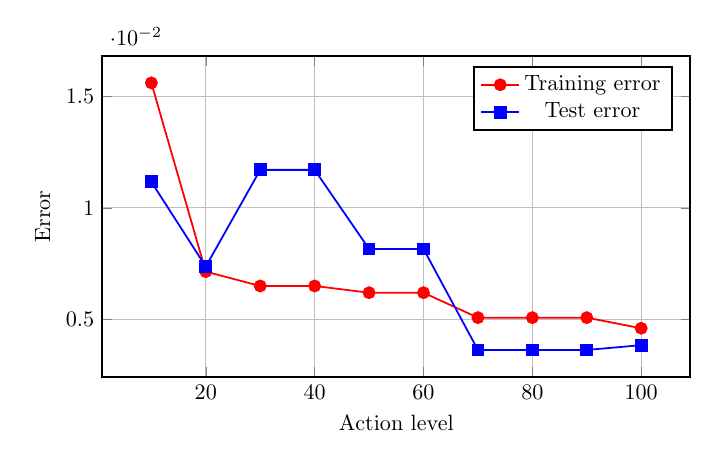
\begin{tikzpicture}[scale=0.8]
\begin{axis}[
    width=0.9\textwidth,
    height=0.55\textwidth,
    xlabel={Action level},
    ylabel={Error},
    grid=major,
    legend pos=north east,
    mark size=2.5pt,
    thick,
]

% Training error
\addplot[
    mark=*, red
]
coordinates {
(10, 0.01560839561553183)
(20, 0.007143234577789102)
(30, 0.0064993987438149185)
(40, 0.0064993987438149185)
(50, 0.0061983356366646526)
(60, 0.0061983356366646526)
(70, 0.005079052840165)
(80, 0.005079052840165)
(90, 0.005079052840165)
(100, 0.004602862316874408)
};
\addlegendentry{Training error}

% Test error
\addplot[
    mark=square*, blue
]
coordinates {
(10, 0.011168871624469456)
(20, 0.0073691533606085905)
(30, 0.011706859986466693)
(40, 0.011706859986466693)
(50, 0.008161420560959528)
(60, 0.008161420560959528)
(70, 0.003629703727390215)
(80, 0.003629703727390215)
(90, 0.003629703727390215)
(100, 0.0038447366811493067)
};
\addlegendentry{Test error}

\end{axis}
\end{tikzpicture}
\caption{Training and test errors as a function of action level.}
\end{figure}

\begin{table}[H]
\centering
\begin{tabular}{ccccc}
\toprule
Number of actions & Train error & Train improv. (\%) & Test error & Test improv. (\%) \\
\midrule
10  & 0.01561 & 0.0  & 0.01117 & 0.0 \\
20  & 0.00714 & 54.2 & 0.00737 & 34.0 \\
30  & 0.00650 & 58.3 & 0.01171 & -4.8 \\
40  & 0.00650 & 58.3 & 0.01171 & -4.8 \\
50  & 0.00620 & 60.3 & 0.00816 & 27.0 \\
60  & 0.00620 & 60.3 & 0.00816 & 27.0 \\
70  & 0.00508 & 67.5 & 0.00363 & 67.5 \\
80  & 0.00508 & 67.5 & 0.00363 & 67.5 \\
90  & 0.00508 & 67.5 & 0.00363 & 67.5 \\
100 & 0.00460 & 70.5 & 0.00384 & 65.6 \\
\bottomrule
\end{tabular}
\caption{Relative improvement compared to number of actions.}
\end{table}

As it is seen, the errors tend to decrease as the number of actions grows. In early stages, we see perturbation in the error of test scores, which is mostly likely due to the random sampling of actions. As a validation of the previous discussion on the limiting effect of actions on states, the next table illustrates the correlation between the duration of training and the action level.

\begin{table}[H]
\centering
\begin{tabular}{cccc}
\toprule
Action level & Training error & Test error & Time (min:sec) \\
\midrule
10  & 0.01561 & 0.01117 & 0:06 \\
20  & 0.00714 & 0.00737 & 0:17 \\
30  & 0.00650 & 0.01171 & 0:35 \\
40  & 0.00650 & 0.01171 & 1:03 \\
50  & 0.00620 & 0.00816 & 1:40 \\
60  & 0.00620 & 0.00816 & 2:17 \\
70  & 0.00508 & 0.00363 & 3:09 \\
80  & 0.00508 & 0.00363 & 4:12 \\
90  & 0.00508 & 0.00363 & 5:27 \\
100 & 0.00460 & 0.00384 & 6:43 \\
\bottomrule
\end{tabular}
\medskip

\caption{Performance versus action level with runtime.}
\end{table}

Moreover, we plot the time-action levels using linear interpolation.


\begin{figure}[H]
\centering
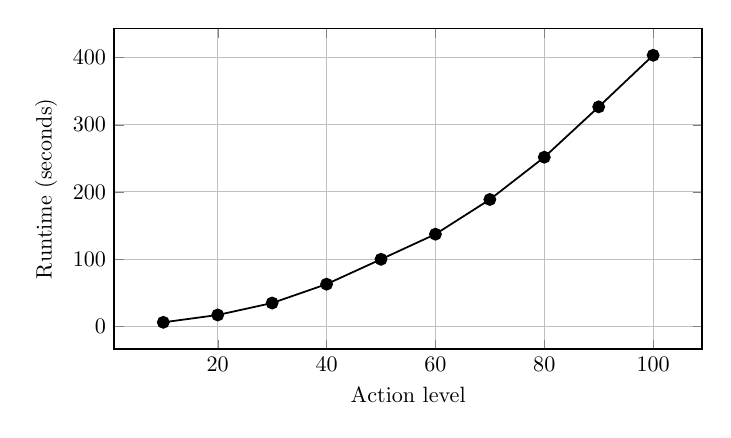
\begin{tikzpicture}[scale=0.8]
\begin{axis}[
    width=0.9\textwidth,
    height=0.55\textwidth,
    xlabel={Action level},
    ylabel={Runtime (seconds)},
    grid=major,
    mark size=2.5pt,
    thick,
]

\addplot[
    mark=*,
]
coordinates {
(10, 5.809951066970825)
(20, 16.74672508239746)
(30, 34.53178596496582)
(40, 62.63665294647217)
(50, 99.69152998924255)
(60, 137.04569816589355)
(70, 188.7130250930786)
(80, 251.65863609313965)
(90, 326.66973209381104)
(100, 403.46485805511475)
};
\end{axis}
\end{tikzpicture}
\caption{Runtime as a function of action level.}
\end{figure}

The best-fitting quadratic function, in the least squares sense, is $P(M) = 0.0437611M^2-0.420042M+7.318885$, where $M$ is the number of actions, with the goodness of fit score $R^2=0.999673$. Therefore, it is possible to say that runtime of training is asymptotically and approximately $0.044M^2$.

To summarize, this toy example exemplifies that the triply quantized training procedure described in this paper leads to near-convergence to optimal controls as the quantization becomes finer.

\section{Conclusion}
In this paper, we formulated Transformers as a discrete-time McKean---Vlasov dynamics system and lifted this dynamics to a measure-valued discrete-time Markov decision process. This lifting yielded the Markov property for the ensemble of probability measures that are obtained from initial data, which allowed us to use the dynamic programming principle to establish near-optimality. Although the optimal policies obtained from dynamic programming principle are of closed-loop nature, we argued that they should be seem as a theoretical tool, but not a practical one. Then we showed that from the deterministic flow of measure-valued MDP and the deterministic nature of closed-loop policies, we can get initial-data-dependent open-loop policies, which are compatible with the orthodox training methods of Transformers by fixing neural network weights after training. Therefore, such policies are the correct abstraction of neural network weights from the perspective of optimal control theory. After that, we proposed a quantization-based learning algorithm, which is compatible with the theory presented in this paper, and we showed that it is possible to get near-optimal policies that are computationally more feasible than running dynamic programming on the infinite-dimensional measure-valued space.

Although, by quantizing, we reduced the infinite-dimensional measure-valued space to a finite-dimensional probability simplex, then to a finite set, the training-by-quantization is not designed as a scalable solver of this problem, but as a helper to conduct numerical experiment that is compatible with the theory. The main contribution of the framework presented is providing another perspective on Transformers to understand its structure better and guarantee the existence of optimal weights for it, rather than providing an efficient and scalable algorithm. Also, the subjects of this paper are not a competitor to gradient-descent-based techniques, however; since many applications of Transformers use gradient-descent methods for, in general, a non-convex and non-differentiable system, which indicates that the underlying structure of Transformers is not really understood. 

The present work so far is mainly theoretical and aiming to provide a structural comprehension of Transformers from the viewpoint of optimal control theory. As for future research directions, it is possible to consider mean-field case ($N\to\infty$) for this formulation and seek connections with mean-field games. Moreover, making the learning process with dynamics programming more tractable is critical since it has problems with high-dimensional data as many MDP-based systems do. We believe that these directions may have a contribution to understand the connections between Transformers and optimal control theory.

\appendix

\section{Auxiliary Results used in Section 4}
In this part, we provide all of the necessary lemmata and correlated results that are used to prove the main results of this section.
\begin{lemma}\label{lemma:f-lipschitz}
    Under Assumption \ref{assume:compactness}, $f$ satisfies the following Lipschitz condition for all $(p,x),(q,y)\in\XX$, $U\in\UU$, and all $\mu,\nu\in\cP(\XX)$
    \begin{equation*}
        \|f((p,x);U;\mu)-f((q,y);U;\nu)\|_{2,\lambda} \leq L_f(\|(p,x)-(q,y)\|_{2,\lambda} + W_{2,\lambda}(\mu,\nu))
    \end{equation*}
    for some $L_f \geq 0$.
\end{lemma}
\begin{proof}
    Since the estimations are tedious, we go step-by-step. First, for fixed $U\in\UU$ and for any $(r,z)\in\XX$ and
    \begin{equation*}
        f((r,z);U,\omega) = \left(r, W(\sigma(Az+b)) + \frac{N(z,\omega)}{D(z,\omega)}\right)
    \end{equation*}
    where $N(z,\omega) := \int_{\mathrm{S}}\omega_{\mathrm S}(\de z^\prime)\e^{\beta\langle Qz, Kz^\prime\rangle}Vz^\prime$ and $D(z, \omega) := \int_{\mathrm S} \omega_{\mathrm S}(\de z^\prime)\e^{\beta\langle Qz, Kz^\prime\rangle}$. By Assumption \ref{assume:compactness}, we have
    \begin{itemize}
        \item $\|N(z,\omega)\| \leq \e^{\beta\|Q\|\|K\|\|z\|^2} \leq \e^{\beta(\operatorname{diam}(\UU)\operatorname{diam}(\mathrm{S}))^2}\operatorname{diam}(\UU)\operatorname{diam}(\mathrm{S}) =: B_N$.
        \item $|D(z,\omega)| \leq \e^{\beta(\operatorname{diam}(\UU)\operatorname{diam}(\mathrm{S}))^2} =: B_D$.
    \end{itemize}
    Since $x\mapsto \e^{\beta\langle Qx, Kz^\prime\rangle}Vz^\prime$ is a smooth function for any $z^\prime\in\mathrm{S}$, it is also a globally Lipschitz function. Write $L_1$ for the corresponding Lipschitz constant. From here, it follows that $N$ and $D$ satisfy the following Lipschitz conditions:
    \begin{align*}
        \|N(x,\mu) - N(y,\nu)\| &= \|N(x,\mu) - N(y, \mu) + N(y,\mu) - N(y,\nu)\| \\
        &\leq \|N(x,\mu) - N(y, \mu)\| + \|N(y,\mu) - N(y,\nu)\|\\
        &= \left\|\int_{\mathrm{S}}\mu_{\mathrm S}(\de z^\prime)(\e^{\beta\langle Qx, Kz^\prime\rangle}- \e^{\beta\langle Qy, Kz^\prime\rangle})Vz^\prime\right\| \\
        &\qquad+ \left\|\int_{\mathrm{S}}\mu_{\mathrm S}(\de z^\prime)\e^{\beta\langle Qy, Kz^\prime\rangle}Vz^\prime - \int_{\mathrm{S}}\nu_{\mathrm S}(\de z^\prime)\e^{\beta\langle Qy, Kz^\prime\rangle}Vz^\prime\right\| \\
        &\leq L_1\operatorname{diam}(\mathrm S)\operatorname{diam}(\UU)\|x-y\| + B \cdot W_{2,\lambda}(\mu,\nu) 
\end{align*}
where the last inequality is obtained as follows: The first summand is a consequence of Lipschitz nature of the map $x\mapsto \e^{\beta\langle Qx, Kz^\prime\rangle}Vz^\prime$. Since both $\mathrm{S}$ and $\UU$ are compact, the map $(Q,K,V,z,z^\prime)\mapsto\e^{\beta\langle Qz, Kz^\prime\rangle}Vz^\prime$ is bounded and say $B$ is the minimal bound. Then,
\begin{align*}
    \left\|\int_{\mathrm{S}}\mu_{\mathrm S}(\de z^\prime)\e^{\beta\langle Qy, Kz^\prime\rangle}Vz^\prime - \int_{\mathrm{S}}\nu_{\mathrm S}(\de z^\prime)\e^{\beta\langle Qy, Kz^\prime\rangle}Vz^\prime\right\| &= B\cdot\bigg\|\int_{\mathrm{S}}\mu_{\mathrm S}(\de z^\prime)\frac{\e^{\beta\langle Qy, Kz^\prime\rangle}Vz^\prime}{B} \\&\hspace{5em}- \int_{\mathrm{S}}\nu_{\mathrm S}(\de z^\prime)\frac{\e^{\beta\langle Qy, Kz^\prime\rangle}Vz^\prime}{B}\bigg\|  \\
    &\leq B\cdot W_1(\mu_\mathrm{S},\nu_\mathrm{S}) \leq B \cdot W_{2,\lambda}(\mu,\nu).
\end{align*}
Here, we normalize the inner function to obtain a function with unit Lipschitz constant. This maneuver enables us to use the dual form of $W_1$ \cite[Remark 6.5]{villani2008optimal}. In addition, we have $W_1(\mu_\mathrm{S},\nu_\mathrm{S}) \leq W_{2,\lambda}(\mu,\nu)$ since $p$-Wasserstein distances increase as $p$ increases \cite[Remark 6.6]{villani2008optimal} and $W_{2}(\mu_\mathrm{S},\nu_\mathrm{S}) \leq W_{2,\lambda}(\mu,\nu)$ as we include the distance between positional encodings to the cost structure.

So, by writing 
\begin{equation*}
    \|N(x,\mu) - N(y,\nu)\| \leq \max\{L_1\operatorname{diam}(\mathrm S)\operatorname{diam}(\UU), B\}(\|x-y\| + W_{2,\lambda}(\mu,\nu))
\end{equation*}
we establish Lipschitz property of $N$. We write $L_N = \max\{L_1\operatorname{diam}(\mathrm S)\operatorname{diam}(\UU), B\}$ in order to be a little bit more concise. With a similar argument, we also have
\begin{equation*}
    |D(x,\mu) - D(y,\nu)| \leq L_D(\|x-y\| + W_{2,\lambda}(\mu,\nu)).
\end{equation*}

Before moving on to estimating $f$, we remind that the compactness assumptions force $D(z,\omega)$ to be bounded away from zero. Write $C_{\text{min}} := \min_{z,\omega}D(z,\omega)$. Then
\begin{align*}
    \left\|\left(W\sigma(Ax + b) - W\sigma(Ay + b) + \frac{N(x,\mu)}{D(x,\mu)} - \frac{N(y,\nu)}{D(y,\nu)}\right)\right\|_{2} &\leq \bigg\| W\sigma(Ax + b) - W\sigma(Ay + b)\bigg\|_{2} \\
    &+\bigg\|\frac{D(y,\mu)N(x,\mu) - D(x,\mu)N(y,\nu)}{D(x,\mu)D(y,\nu)}\bigg\|_{2}\\
    &\leq \|W\|\cdot\|A\|\cdot\operatorname{Lip}(\sigma)\cdot\|x-y\|_{2}\\
    &\qquad+\frac{1}{C_{\text{min}}^2}\left\|(D(y,\nu) - D(x,\mu))N(x,\mu)\right\|_{2}\\
    &\qquad+\frac{1}{C_{\text{min}}^2}\left\|D(x,\mu)(N(x,\mu) - N(y,\nu))\right\|_{2}\\
    &\leq \operatorname{diam}(\UU)^2\|x-y\|_{2}\\
    &+ \frac{1}{C_{\text{min}}^2}(L_DB_N + L_NB_D)(\|x-y\|_2 \\
    &\hspace{10em}+ W_{2,\lambda}(\mu,\nu)).
\end{align*}
Letting $L_2 := \operatorname{diam}(\UU)^2(L_DB_N + L_NB_D)C_{\text{min}}^{-2}$, we get
\begin{equation*}
    \left\|\left(W\sigma(Ax + b) - W\sigma(Ay + b) + \frac{N(x,\mu)}{D(x,\mu)} - \frac{N(y,\nu)}{D(y,\nu)}\right)\right\|_{2} \leq L_2(\|x-y\|_2 + W_{2,\lambda}(\mu,\nu)).
\end{equation*}
Consequently,
\begin{align*}
    \|f(p,x;U,\mu)-f(p,y;,U,\nu)\|_{2,\lambda} &= \left\|\left(W\sigma(Ax + b) - W\sigma(Ay + b) + \frac{N(x,\mu)}{D(x,\mu)} - \frac{N(y,\nu)}{D(y,\nu)}\right)\right\|_{2}\\
    &\leq L_2(\|x-y\|_2 + W_{2,\lambda}(\mu,\nu)).
\end{align*}
A simple application of quadratic mean-arithmetic mean inequality and sub-additivity of square root gives us:
    \begin{align*}
        \|f(X;U;\mu) - f(Y; U; \nu)\|_{2,\lambda} &\leq \sqrt{\lambda|p-q|^2 + L_2(\|x-y\|_2 + W_{2,\lambda}(\mu,\nu))^2}\\
        &\leq \sqrt{\lambda|p-q|^2 + 2L_2(\|x-y\|_2^2 + W_{2,\lambda}(\mu,\nu)^2)}\\
        &\leq \max\{1, \sqrt{2L_2}\}\sqrt{(\lambda|p-q|^2 + \|x-y\|_2^2) + W_{2,\lambda}(\mu,\nu)^2}\\
        &\leq \max\{1, \sqrt{2L_2}\}(\|(p,q)-(q,y)\|_{2,\lambda} + W_{2,\lambda}(\mu,\nu)).
    \end{align*}
\end{proof}
From now on, we write $L_f$ for $\max\{1, \sqrt{2L_2}\}$ in order to make the notation easier to follow. The Lipschitz nature of $f$ and the compositional structure of the flow map $\Phi$ yield us the following Lipschitz type estimate, which comes handy while showing the convergence of the quantized problem to the original one.
\begin{corollary}\label{cor:phi-lipschitz}
    For any $\bm{\mu},\bm{\nu}\in\cP(\XX)^K$ and $U\in\UU$, we have
    \begin{equation*}
        \sum_{k=1}^K W_{2,\lambda}(\Phi(\mu^k,U), \Phi(\nu^k, U)) \leq L_\Phi \sum_{k=1}^KW_{2,\lambda}(\mu^k,\nu^k)
    \end{equation*}
    for some $L_\Phi \geq 0$. We here write $\bm{\mu} = (\mu^1,\ldots,\mu^K)$ and $\bm{\nu} = (\nu^1,\ldots,\nu^K)$.
\end{corollary}
\begin{proof}
    We prove the simple case $K=1$, from which the general case follows. Indeed, let $\mu,\nu\in\cP(\XX)$ and $U\in\UU$, then let $\pi^*$ be an $W_{2,\lambda}$-optimal coupling of $\Phi(\mu,U)$ and $\Phi(\nu, U)$. Define
    \begin{equation*}
        \tilde{\pi}(\de(\tilde{p},\tilde{x}),\de(\tilde{q}, \tilde{y})) := \pi^*(f^{-1}(\de(\tilde{p},\tilde{x}), U, \mu), f^{-1}(\de(\tilde{q}, \tilde{y}), U, \nu)).
    \end{equation*}
    By a change of variables argument and by Lemma \ref{lemma:f-lipschitz}, we get
    \begin{align*}
        W_{2,\lambda}(\Phi(\mu,U), \Phi(\nu, U))^2 &\leq \int_{\XX\times\XX} \tilde{\pi}(\de(\tilde{p},\tilde{x}),\de(\tilde{q},\tilde{y})) \|(\tilde{p},\tilde{x})-(\tilde{q}, \tilde{y})\|_{2,\lambda}^2\\
        &\leq\int_{\XX\times\XX}\pi^*(\de(p,x), \de(q,y))\|f((p,x);U;\mu)-f((q,y);U;\nu)\|_{2,\lambda}^2\\
        &\leq L_f^2\int_{\XX\times\XX}\pi^*(\de(p,x), \de(q,y))(\|(p,x)-(q,y)\|_{2,\lambda}^2 + W_{2,\lambda}(\mu,\nu)^2)\\
        &=2L_f^2 W_{2,\lambda}(\mu,\nu)^2.
    \end{align*}
    Thus, writing $L_\Phi := \sqrt{2}L_f$,
    \begin{equation*}
        W_{2,\lambda}(\Phi(\mu,U), \Phi(\nu, U)) \leq L_\Phi W_{2,\lambda}(\mu,\nu).
    \end{equation*}
\end{proof}

\begin{lemma}\label{lemma:approximate-measure}
    Let $\mu\in\cP(\XX)$. Then $W_{2,\lambda}(\mu,\mu\circ (Q^{(n)})^{-1}) < \frac{1}{n}$.
\end{lemma}
\begin{proof}
    Let $\pi$ be a coupling for the law of $((p,x), Q^{(n)}((p,x)))$ with $(p,x)\sim\mu\in\cP(\XX)$. Then,
    \begin{align*}
        W_{2,\lambda}(\mu,\mu\circ (Q^{(n)})^{-1})^2 &\leq \int_{\XX\times\XX}\pi(\de(p,x), \de (q,y))\|(p,x)-(q,y)\|_{2,\lambda}^2\\
        &\leq \EE_{(p,x)\sim\mu}\|(p,x)-Q^{(n)}((p,x))\|_{2,\lambda}^2\\
        &\leq \int_{\XX\times\XX}\pi(\de (p,x), \de (q,y))\frac{1}{n^2}.
    \end{align*}
    In the last inequality, we use $\|(p,x)-Q^{(n)}((p,x))\|_{2,\lambda} \leq \frac{1}{n}$, given by the definition of $(Q^{(n)})^{-1}$. Thus, $W_{2,\lambda}(\mu,\mu\circ (Q^{(n)})^{-1}) \leq \frac{1}{n}$.
\end{proof}

\begin{corollary}\label{cor:lipschitz-phi_n}
    For all $n\in\NN$, there is $L_{\Phi^{(n)}} \geq 0$ such that for all $\bar{\mu},\bar{\nu}\in\cP(\XX_n)$ and $U\in\UU$, we have
    \begin{equation*}
        W_{2,\lambda}(\Phi^{(n)}(\bar{\mu}, U), \Phi^{(n)}(\bar{\nu}, U)) \leq L_{\Phi^{(n)}}W_{2,\lambda}(\bar{\mu},\bar{\nu}).
    \end{equation*}
\end{corollary}
\begin{proof}
    Let $\pi^*$ be an optimal coupling between $\Phi^{(n)}(\bar{\mu}, U)$ and $\Phi^{(n)}(\bar{\nu}, U)$. We define
    \begin{equation*}
        \tilde{\pi}(\de(\tilde{p},\tilde{x}), \de(\tilde{q},\tilde{y})) := \pi^*(f_n^{-1}(\de(\tilde{p},\tilde{x}), U, \bar{\mu}), f_n^{-1}(\de(\tilde{q},\tilde{y}), U, \bar{\nu})).
    \end{equation*}
    Then
    \begin{align*}
        W_{2,\lambda}(\Phi^{(n)}(\bar{\mu}, U), \Phi^{(n)}(\bar{\nu}, U))^2 &\leq \int_{\XX\times\XX}\tilde{\pi}(\de(\tilde{p},\tilde{x}), \de(\tilde{q},\tilde{y}))\|(\tilde{p},\tilde{x})-(\tilde{q},\tilde{y})\|_{2,\lambda}^2\\
        &\leq\int_{\XX\times\XX}\pi^*(\de(p,x), \de (q,y))\|f_n((p,x); U, \bar{\mu})- f_n((q,y); U, \bar{\nu})\|_{2,\lambda}^2\\
        &\leq \int_{\XX\times\XX}\pi^*(\de(p,x), \de (q,y))\|f((p,x); U, \bar{\mu})-f((q,y); U, \bar{\nu})\|_{2,\lambda}^2\\
        &\leq L_f^2\int_{\XX\times\XX}\pi^*(\de(p,x), \de (q,y))(\|(p,x)-(q,y)\|_{2,\lambda}^2 + W_{2,\lambda}(\bar{\mu},\bar{\nu})^2)\\
        &\leq 2L_f^2W_{2,\lambda}(\bar{\mu},\bar{\nu})^2.
    \end{align*}
    In these estimations, we use Lemma \ref{lemma:f-lipschitz} and use the fact that $\|Q^{(n)}(p,x) - Q^{(n)}(q,y)\|_{2,\lambda} \leq \|(p,x) - (q,y)\|_{2,\lambda}$, which is evident by the definition of $Q^{(n)}$ and the reverse triangle inequality.
\end{proof}

\acks{This research has been partially supported by the Turkish Academy of Sciences through the 2025 GEBIP Award, and by the Natural Sciences and Engineering Research Council of Canada (NSERC)}

%\bibliographystyle{amsplain}
\begin{thebibliography}{43}
\providecommand{\natexlab}[1]{#1}
\providecommand{\url}[1]{\texttt{#1}}
\expandafter\ifx\csname urlstyle\endcsname\relax
  \providecommand{\doi}[1]{doi: #1}\else
  \providecommand{\doi}{doi: \begingroup \urlstyle{rm}\Url}\fi

\bibitem[Achiam et~al.(2023)Achiam, Adler, Agarwal, Ahmad, Akkaya, Aleman, Almeida, Altenschmidt, Altman, Anadkat, et~al.]{achiam2023gpt}
J.~Achiam, S.~Adler, S.~Agarwal, L.~Ahmad, I.~Akkaya, F.~L. Aleman, D.~Almeida, J.~Altenschmidt, S.~Altman, S.~Anadkat, et~al.
\newblock {GPT}-4 technical report.
\newblock \emph{arXiv preprint arXiv:2303.08774}, 2023.

\bibitem[Allen-Zhu et~al.(2019)Allen-Zhu, Li, and Liang]{allen2019learning}
Z.~Allen-Zhu, Y.~Li, and Y.~Liang.
\newblock Learning and generalization in overparameterized neural networks, going beyond two layers.
\newblock \emph{Advances in neural information processing systems}, 32, 2019.

\bibitem[Arora et~al.(2018)Arora, Cohen, Golowich, and Hu]{arora2018convergence}
S.~Arora, N.~Cohen, N.~Golowich, and W.~Hu.
\newblock A convergence analysis of gradient descent for deep linear neural networks.
\newblock \emph{arXiv preprint arXiv:1810.02281}, 2018.

\bibitem[B{\"a}uerle(2023)]{bauerle2023mean}
N.~B{\"a}uerle.
\newblock Mean field {Markov} decision processes.
\newblock \emph{Applied mathematics \& optimization}, 88\penalty0 (1):\penalty0 12, 2023.

\bibitem[Bayraktar et~al.(2018)Bayraktar, Cosso, and Pham]{bayraktar2018randomized}
E.~Bayraktar, A.~Cosso, and H.~Pham.
\newblock Randomized dynamic programming principle and {F}eynman-{K}ac representation for optimal control of {M}c{K}ean---{V}lasov dynamics.
\newblock \emph{Transactions of the American Mathematical Society}, 370\penalty0 (3):\penalty0 2115--2160, 2018.

\bibitem[Benning et~al.(2021)Benning, Celledoni, Ehrhardt, Owren, and Schönlieb]{benning2021}
M.~Benning, E.~Celledoni, M.~J. Ehrhardt, B.~Owren, and C.-B. Schönlieb.
\newblock Deep learning as optimal control problems.
\newblock \emph{IFAC-PapersOnLine}, 54\penalty0 (9):\penalty0 620--623, 2021.
\newblock ISSN 2405-8963.
\newblock \doi{https://doi.org/10.1016/j.ifacol.2021.06.124}.
\newblock URL \url{https://www.sciencedirect.com/science/article/pii/S2405896321006029}.
\newblock 24th International Symposium on Mathematical Theory of Networks and Systems MTNS 2020.

\bibitem[Billingsley(2013)]{billingsley2013convergence}
P.~Billingsley.
\newblock \emph{Convergence of probability measures}.
\newblock John Wiley \& Sons, 2013.

\bibitem[Blackwell(1964)]{blackwell1964memoryless}
D.~Blackwell.
\newblock Memoryless strategies in finite-stage dynamic programming.
\newblock \emph{The Annals of Mathematical Statistics}, 35\penalty0 (2):\penalty0 863--865, 1964.

\bibitem[Boyd and Vandenberghe(2004)]{boyd2004convex}
S.~Boyd and L.~Vandenberghe.
\newblock \emph{Convex optimization}.
\newblock Cambridge university press, 2004.

\bibitem[Carmona and Delarue(2015)]{carmona2015forward}
R.~Carmona and F.~Delarue.
\newblock Forward--backward stochastic differential equations and controlled {McKean--Vlasov} dynamics.
\newblock 2015.

\bibitem[Carmona et~al.(2013)Carmona, Delarue, and Lachapelle]{carmona2013control}
R.~Carmona, F.~Delarue, and A.~Lachapelle.
\newblock Control of {McKean--Vlasov} dynamics versus mean field games.
\newblock \emph{Mathematics and Financial Economics}, 7\penalty0 (2):\penalty0 131--166, 2013.

\bibitem[Carmona et~al.(2023)Carmona, Lauri{\`e}re, and Tan]{carmona2023model}
R.~Carmona, M.~Lauri{\`e}re, and Z.~Tan.
\newblock Model-free mean-field reinforcement learning: mean-field {MDP} and mean-field {Q}-learning.
\newblock \emph{The Annals of Applied Probability}, 33\penalty0 (6B):\penalty0 5334--5381, 2023.

\bibitem[Castin et~al.(2025)Castin, Ablin, Carrillo, and Peyr{\'e}]{castin2025unified}
V.~Castin, P.~Ablin, J.~A. Carrillo, and G.~Peyr{\'e}.
\newblock A unified perspective on the dynamics of deep {T}ransformers.
\newblock \emph{arXiv preprint arXiv:2501.18322}, 2025.

\bibitem[Chen et~al.(2018)Chen, Rubanova, Bettencourt, and Duvenaud]{chen2018neural}
R.~T. Chen, Y.~Rubanova, J.~Bettencourt, and D.~K. Duvenaud.
\newblock Neural ordinary differential equations.
\newblock \emph{Advances in neural information processing systems}, 31, 2018.

\bibitem[Cohn(2013)]{cohn2013measure}
D.~L. Cohn.
\newblock \emph{Measure theory}, volume~1.
\newblock Springer, 2013.

\bibitem[Conway(1994)]{conway1994course}
J.~B. Conway.
\newblock \emph{A course in functional analysis}, volume~96.
\newblock Springer Science \& Business Media, 1994.

\bibitem[Du et~al.(2018)Du, Zhai, Poczos, and Singh]{du2018gradient}
S.~S. Du, X.~Zhai, B.~Poczos, and A.~Singh.
\newblock Gradient descent provably optimizes over-parameterized neural networks.
\newblock \emph{arXiv preprint arXiv:1810.02054}, 2018.

\bibitem[E et~al.(2019)E, Ma, and Wu]{E2019}
W.~E, C.~Ma, and L.~Wu.
\newblock A mean-field optimal control formulation of deep learning.
\newblock \emph{Research in the Mathematical Sciences}, 6\penalty0 (1):\penalty0 1--41, 2019.
\newblock \doi{10.1007/s40687-019-0172-7}.

\bibitem[Geshkovski et~al.(2023)Geshkovski, Letrouit, Polyanskiy, and Rigollet]{geshkovski2023emergence}
B.~Geshkovski, C.~Letrouit, Y.~Polyanskiy, and P.~Rigollet.
\newblock The emergence of clusters in self-attention dynamics.
\newblock \emph{Advances in Neural Information Processing Systems}, 36:\penalty0 57026--57037, 2023.

\bibitem[Geshkovski et~al.(2025)Geshkovski, Letrouit, Polyanskiy, and Rigollet]{geshkovski2025mathematical}
B.~Geshkovski, C.~Letrouit, Y.~Polyanskiy, and P.~Rigollet.
\newblock A mathematical perspective on {T}ransformers.
\newblock \emph{Bulletin of the American Mathematical Society}, 62\penalty0 (3):\penalty0 427--479, 2025.

\bibitem[Haber and Ruthotto(2017)]{haber2017stable}
E.~Haber and L.~Ruthotto.
\newblock Stable architectures for deep neural networks.
\newblock \emph{Inverse problems}, 34\penalty0 (1):\penalty0 014004, 2017.

\bibitem[Hern{\'a}ndez-Lerma and Lasserre(2012)]{hernandez2012discrete}
O.~Hern{\'a}ndez-Lerma and J.~B. Lasserre.
\newblock \emph{Discrete-time {Markov} control processes: basic optimality criteria}, volume~30.
\newblock Springer Science \& Business Media, 2012.

\bibitem[Hornik et~al.(1989)Hornik, Stinchcombe, and White]{hornik1989multilayer}
K.~Hornik, M.~Stinchcombe, and H.~White.
\newblock Multilayer feedforward networks are universal approximators.
\newblock \emph{Neural networks}, 2\penalty0 (5):\penalty0 359--366, 1989.

\bibitem[Li and Khaneja(2009)]{li2009ensemble}
J.-S. Li and N.~Khaneja.
\newblock Ensemble control of bloch equations.
\newblock \emph{IEEE Transactions on Automatic Control}, 54\penalty0 (3):\penalty0 528--536, 2009.

\bibitem[Li et~al.(2018)Li, Chen, Tai, et~al.]{li2018maximum}
Q.~Li, L.~Chen, C.~Tai, et~al.
\newblock Maximum principle based algorithms for deep learning.
\newblock \emph{Journal of Machine Learning Research}, 18\penalty0 (165):\penalty0 1--29, 2018.

\bibitem[Lugosi and Neu(2022)]{lugosi2022generalization}
G.~Lugosi and G.~Neu.
\newblock Generalization bounds via convex analysis.
\newblock In \emph{Proceedings of the 35th Annual Conference on Learning Theory (COLT 2022)}, volume 178 of \emph{Proceedings of Machine Learning Research}, pages 1--23. PMLR, 2022.

\bibitem[McKean~Jr(1966)]{mckean1966class}
H.~P. McKean~Jr.
\newblock A class of {M}arkov processes associated with nonlinear parabolic equations.
\newblock \emph{Proceedings of the National Academy of Sciences}, 56\penalty0 (6):\penalty0 1907--1911, 1966.

\bibitem[Motte and Pham(2022)]{motte2022mean}
M.~Motte and H.~Pham.
\newblock Mean-field {Markov} decision processes with common noise and open-loop controls.
\newblock \emph{The Annals of Applied Probability}, 32\penalty0 (2):\penalty0 1421--1458, 2022.

\bibitem[Mwigo and Dasgupta(2025)]{mwigo2025generalization}
B.~Mwigo and A.~Dasgupta.
\newblock Generalization bound for a shallow transformer trained using gradient descent.
\newblock \emph{Transactions on Machine Learning Research}, December 2025.
\newblock URL \url{https://openreview.net/forum?id=t3iUeMOT8Z}.
\newblock Published 12/2025.

\bibitem[Pham and Wei(2016)]{pham2016discrete}
H.~Pham and X.~Wei.
\newblock Discrete time {McKean--Vlasov} control problem: a dynamic programming approach.
\newblock \emph{Applied Mathematics \& Optimization}, 74\penalty0 (3):\penalty0 487--506, 2016.

\bibitem[Pham and Wei(2017)]{pham2017dynamic}
H.~Pham and X.~Wei.
\newblock Dynamic programming for optimal control of stochastic {McKean--Vlasov} dynamics.
\newblock \emph{SIAM Journal on Control and Optimization}, 55\penalty0 (2):\penalty0 1069--1101, 2017.

\bibitem[Phuong and Hutter(2022)]{phuong2022formal}
M.~Phuong and M.~Hutter.
\newblock Formal algorithms for {T}ransformers.
\newblock \emph{arXiv preprint arXiv:2207.09238}, 2022.

\bibitem[Pradhan and Y\"uksel(2025)]{PY25MckeanVA}
S.~Pradhan and S.~Y\"uksel.
\newblock Near optimality of discrete-time approximations for controlled {McKean---Vlasov} diffusions and interacting particle systems.
\newblock \emph{arXiv preprint arXiv:2510.21208}, 2025.

\bibitem[Reznik(2011)]{reznik2011algorithm}
Y.~A. Reznik.
\newblock An algorithm for quantization of discrete probability distributions.
\newblock In \emph{2011 Data Compression Conference}, pages 333--342. IEEE, 2011.

\bibitem[Ruiz-Balet and Zuazua(2023)]{ruiz2023neural}
D.~Ruiz-Balet and E.~Zuazua.
\newblock Neural {ODE} control for classification, approximation, and transport.
\newblock \emph{SIAM Review}, 65\penalty0 (3):\penalty0 735--773, 2023.

\bibitem[Ruthotto and Haber(2020)]{ruthotto2020deep}
L.~Ruthotto and E.~Haber.
\newblock Deep neural networks motivated by partial differential equations.
\newblock \emph{Journal of Mathematical Imaging and Vision}, 62\penalty0 (3):\penalty0 352--364, 2020.

\bibitem[Sanjari et~al.(2025)Sanjari, Saldi, and Yüksel]{sanjari2025optimalitysymmetricindependentpolicies}
S.~Sanjari, N.~Saldi, and S.~Yüksel.
\newblock Optimality of symmetric independent policies under decentralized mean-field information sharing for stochastic teams and equivalence with {McKean---Vlasov} control of a representative agent, 2025.
\newblock URL \url{https://arxiv.org/abs/2404.04957}.

\bibitem[Vaswani et~al.(2017)Vaswani, Shazeer, Parmar, Uszkoreit, Jones, Gomez, Kaiser, and Polosukhin]{vaswani2017attention}
A.~Vaswani, N.~Shazeer, N.~Parmar, J.~Uszkoreit, L.~Jones, A.~N. Gomez, {\L}.~Kaiser, and I.~Polosukhin.
\newblock Attention is all you need.
\newblock \emph{Advances in neural information processing systems}, 30, 2017.

\bibitem[Villani(2008)]{villani2008optimal}
C.~Villani.
\newblock \emph{Optimal transport: old and new}, volume 338.
\newblock Springer, 2008.

\bibitem[Weinan(2017)]{weinan2017proposal}
E.~Weinan.
\newblock A proposal on machine learning via dynamical systems.
\newblock \emph{Communications in Mathematics and Statistics}, 5\penalty0 (1):\penalty0 1--11, 2017.

\bibitem[Xu and Raginsky(2017)]{xu2017information}
A.~Xu and M.~Raginsky.
\newblock Information-theoretic analysis of generalization capability of learning algorithms.
\newblock In \emph{Advances in Neural Information Processing Systems (NeurIPS 2017)}, Long Beach, CA, USA, 2017. Curran Associates, Inc.

\bibitem[Y{\"u}ksel and Ba{\c{s}}ar(2024)]{yuksel2024stochastic}
S.~Y{\"u}ksel and T.~Ba{\c{s}}ar.
\newblock \emph{Stochastic teams, games, and control under information constraints}.
\newblock Springer, 2024.

\bibitem[Yun et~al.(2019)Yun, Bhojanapalli, Rawat, Reddi, and Kumar]{yun2019transformers}
C.~Yun, S.~Bhojanapalli, A.~S. Rawat, S.~J. Reddi, and S.~Kumar.
\newblock Are {T}ransformers universal approximators of sequence-to-sequence functions?
\newblock \emph{arXiv preprint arXiv:1912.10077}, 2019.

\end{thebibliography}

\end{document}
